\PassOptionsToPackage{T1}{fontenc}
\documentclass[preprint,12pt]{elsarticle}

\usepackage{lmodern}
\usepackage{microtype}

\usepackage{amsmath}
\usepackage{amssymb}
\usepackage{graphicx}
\usepackage{hyperref}
\hypersetup{
	colorlinks=true,
	urlcolor=black,
	citecolor=blue,
	hypertexnames=false,
	pdftitle={Edge-Native Resilient Energy Management for Microgrids Under Network Uncertainty and Power Constraints},
	pdfauthor={Ercan Erkalkan}}
\makeatletter
\pdfstringdefDisableCommands{%
  \def\corref#1{}%
  \def\cnotenum#1{}%
  \def\@corref#1{}%
  \def\texttt#1{#1}%
}
\makeatother
\usepackage[utf8]{inputenc}
\usepackage[english]{babel}
\usepackage{cleveref}
\usepackage[dvipsnames]{xcolor}
\usepackage{booktabs}
\usepackage{array}
\usepackage{algorithm}
\usepackage{algpseudocode}
\usepackage{tabularx}
\usepackage{placeins}
\usepackage{enumitem}
\usepackage{amsthm}
\newtheorem{proposition}{Proposition}

\newcolumntype{Y}{>{\raggedright\arraybackslash}X}

\newcommand{\Rmax}{R_{\max}}
\newcommand{\SOC}{\mathrm{SOC}}
\newcommand{\Pbatt}{P_{\mathrm{batt}}}
\newcommand{\Pcmd}{P_{\mathrm{cmd}}}     
\newcommand{\Pref}{P_{\mathrm{ref}}}    
\newcommand{\Pgrid}{P_{\mathrm{grid}}}
\newcommand{\Pbase}{P_{\mathrm{base}}}
\newcommand{\Pload}{P_{\mathrm{L}}}
\newcommand{\Pres}{P_{\mathrm{RES}}}
\newcommand{\Ppv}{P_{\mathrm{PV}}}
\newcommand{\Pwind}{P_{\mathrm{W}}}
\newcommand{\Pnet}{P_{\mathrm{net}}}
\newcommand{\MA}{\mathrm{MA}}
\newcommand{\EFC}{\mathrm{EFC}}
\newcommand{\Ts}{T_s}
\newcommand{\EFCrf}{\mathrm{EFC}_{\mathrm{rf}}}
\newcommand{\Nmicro}{N_{\mathrm{micro}}}
\newcommand{\dmc}{\delta_{\mathrm{mc}}}
\newcommand{\Hrg}{H_{\mathrm{rg}}}
\newcommand{\Dlim}{\Delta_{\lim}}
\newcommand{\Ecrit}{E_{\mathrm{crit}}}
\newcommand{\Ecritabs}{E_{\mathrm{crit}}^{\mathrm{abs}}}
\newcommand{\gammacrit}{\gamma_{\mathrm{crit}}}
\DeclareMathOperator{\clip}{clip}

\begin{document}

\begin{frontmatter}

\title{Edge-Native Resilient Energy Management for Microgrids Under Network Uncertainty and Power Constraints} %% Article title

\author[Ercan]{Ercan Erkalkan\corref{cor1}}
\cortext[cor1]{Corresponding author. E-mail: \texttt{ercan.erkalkan@marmara.edu.tr}}

\affiliation[Ercan]{
  organization={Department of Computer Technologies, Vocational School of Technical Sciences, Marmara University},
  addressline={Mehmet Genc Campus, Vocational School},
  city={Istanbul},
  postcode={34865},
  country={Turkey}
}

\begin{abstract}
The integration of Distributed Energy Resources (DERs) in modern microgrids heavily relies on Model Predictive Control (MPC) and Cloud-centric optimization. While these approaches offer theoretically optimal dispatch, they suffer from high computational complexity ($\mathcal{O}(N^3)$ solvers) and extreme vulnerability to Internet of Things (IoT) network disruptions, such as packet loss and cloud disconnection. In this paper, we propose a lightweight, Edge-native heuristic Energy Management System (EMS) designed for resource-constrained Edge controllers (e.g., PLCs, Raspberry Pi). The proposed cyber-physical architecture explicitly decouples critical, real-time power cap and battery stress management from Cloud dependencies. We introduce a novel Cyber-Physical Network Uncertainty Model to evaluate EMS controllers under stochastic IoT network disconnection events. Extensive cyber-physical simulations demonstrate that while Cloud-dependent MPC experiences cap-violation exposure (mean 2.38\% across primary benchmark scenarios) due to its online solver dependency, the proposed Edge controller achieves a 100.0\% Resilience Score under both low (2\%) and high (10\%) IoT dropout rates. Furthermore, since the look-back window $w_f$ and forecast horizon $K$ are fixed constants, the Edge-native heuristic executes in $\mathcal{O}(w_f{+}K)=\mathcal{O}(1)$ time per tick, reducing computational overhead by orders of magnitude (microseconds vs.\ milliseconds) compared to state-of-the-art convex optimizers, demonstrating its practical advantage for robust, Next-Generation Smart Grid deployments.
\end{abstract}

\begin{graphicalabstract}
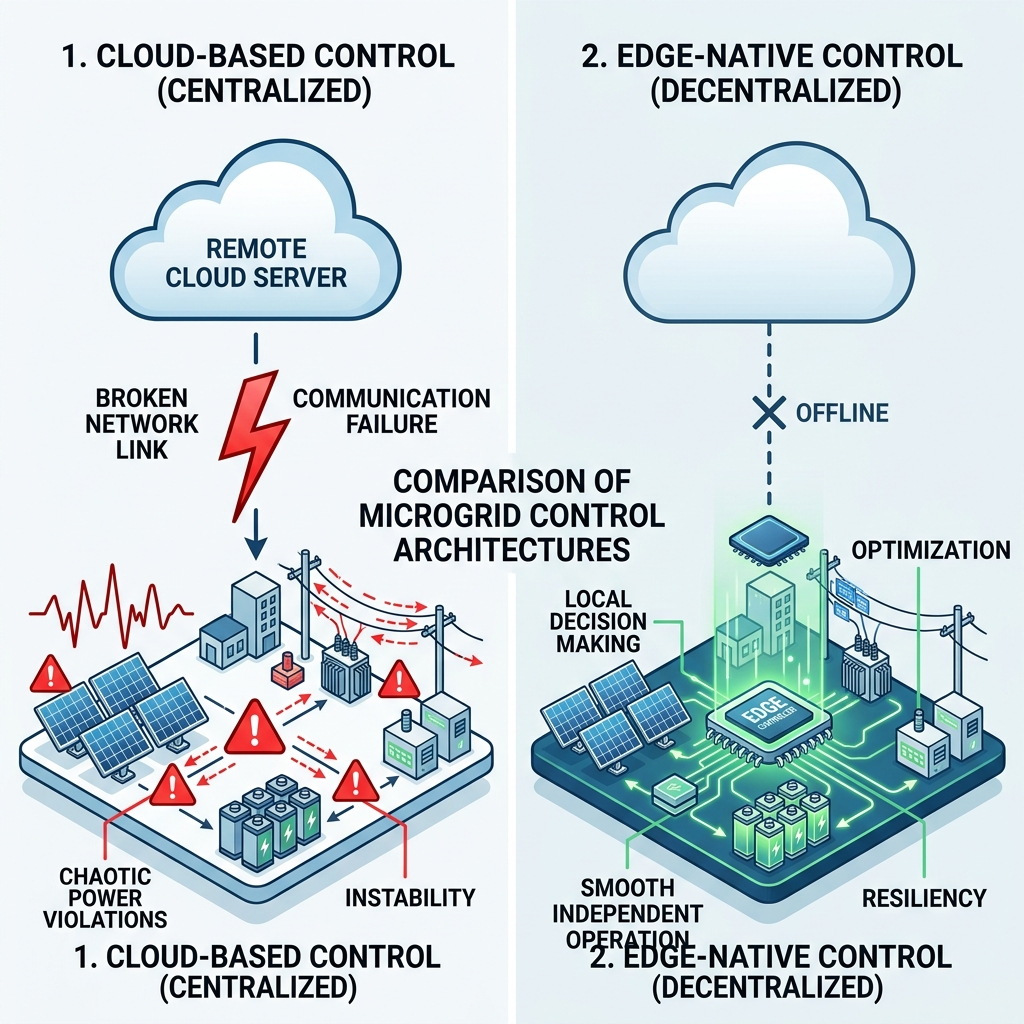
\includegraphics[width=\textwidth]{figures/FGCS_graphical_abstract.png}
\end{graphicalabstract}

%%Research highlights
\begin{highlights}
\item Edge-native EMS with $\mathcal{O}(w_f{+}K)=\mathcal{O}(1)$ per-tick complexity for fixed look-ahead constants.
\item Novel Cyber-Physical Network Uncertainty Model injecting stochastic IoT disconnection events.
\item Edge heuristic achieves 100.0\% Resilience Score under 2\% and 10\% IoT dropout rates.
\item Cloud-MPC incurs mean 2.38\% cap-violation exposure across primary benchmark; Edge: 0.00\%.
\item Sub-millisecond execution: Proposed 0.29--0.35\,ms/tick mean (across benchmark tiers); MPC\_ref 813--1179\,ms/tick mean, p95 up to 1720\,ms/tick.
\end{highlights}

%% Keywords
\begin{keyword}
Edge Computing\sep Internet of Things\sep Cyber-Physical Systems\sep Network Resilience\sep Microgrid EMS\sep Bounded-time computing
\end{keyword}

\end{frontmatter}

\section{Introduction}
The transition toward decentralized Smart Grids has accelerated the deployment of Microgrids equipped with photovoltaic (PV) generation, wind turbines, and Battery Energy Storage Systems (BESS) \cite{lasseter2002microgrids,parhizi2015state}. To manage these complex components, Energy Management Systems (EMS) have traditionally relied on Cloud computing and heavy optimization algorithms, predominantly Model Predictive Control (MPC) and Mixed-Integer Linear Programming (MILP) \cite{hu2021,rawlings2009model}.

However, the next generation of computing systems faces a paradigm shift from Cloud to Edge Computing, driven by the critical limitations of Cloud-dependent architectures in real-time cyber-physical systems (CPS). These limitations include:
1. \textbf{Network Vulnerability:} IoT communication channels between the Edge sensors (meters, BESS) and the Cloud solver are susceptible to jitter, latency, and complete disconnections \cite{ding2019cyber,setiawan2021iot}. When the cloud link fails, traditional MPC is unable to compute the next dispatch vector, leading to severe power cap violations at the point of common coupling (PCC).
2. \textbf{Computational Overhead:} Running predictive optimization solvers requires substantial RAM and CPU capabilities ($\mathcal{O}(N^3)$ for interior-point convex QP solvers), making them entirely unsuited for low-power, localized Edge hardware like Programmable Logic Controllers (PLCs) or embedded single-board computers. Edge computing provides the infrastructure paradigm for moving compute to the device boundary \cite{shi2011survey,mao2017survey}.

The unresolved gap for the present application is therefore not merely another objective term or another solver variant; it is an auditable Edge-native supervisory computing artifact whose online path is explicit, low-compute, and resilient to network disconnections.

This paper addresses these gaps by proposing an Edge-native heuristic controller. Unlike traditional Cloud-based optimization, our approach requires no heavy matrix inversions, running locally with $\mathcal{O}(w_f{+}K)=\mathcal{O}(1)$ per-tick time complexity for fixed look-ahead constants (see Proposition~\ref{prop:fgcrp} in \S\ref{sec:mode_logic}), while aggressively protecting the battery from cyclic stress and preventing grid power-cap violations.

\subsection{Related work and contributions}
\label{sec:related}
\paragraph*{Edge Computing and IoT in Smart Grids.}
The integration of IoT and Edge computing into Smart Grids is a rapidly evolving field, particularly as documented in \emph{Future Generation Computer Systems}. Microgrids themselves have matured from isolated concepts \cite{lasseter2002microgrids,ton2012us} to nationally supported infrastructure programs \cite{parhizi2015state}. The architectural shift from centralized cloud to distributed edge resilience has been established as a central systems concern \cite{taufer2023edge}. Bridging cloud-based high-performance computing with resource-constrained IoT devices broadens the deployment view \cite{taufer2021cloud}. Furthermore, IoT-enabled smart microgrid frameworks reinforce the observability requirement \cite{wang2024fgcs}. Network uncertainty and distributed control in cyber-physical power systems add a critical communication perspective \cite{chen2023fgcs}; unlike \cite{chen2023fgcs}, the present work specifically models the impact of disconnection events on the EMS dispatch layer rather than at the communication protocol level. Bounded-time task scheduling for edge nodes \cite{liu2025fgcs} motivates the fixed-complexity design, extended here to the real-time supervisory control setting.

\paragraph*{Cyber-Physical Resilience and Network Disruption.}
While Edge architectures offer localized execution, microgrids remain cyber-physical systems vulnerable to communication faults \cite{ding2019cyber}. IoT communication degradation directly impacts EMS dispatch quality, as intermittent connectivity compromises the optimality of cloud-computed set-points \cite{setiawan2021iot}. Smart-grid co-simulation provides related cyber--physical evidence. Yet, many microgrid EMS studies prioritize optimization richness (e.g., stochastic MPC \cite{parisio2014model}, two-timescale optimization \cite{li2025twotimescale}, or learning-based dispatch \cite{yang2025shieldeddrl}) while leaving data-dependent solve time, network reliance, and controller auditability in the background.

\paragraph*{Auditable and explainable rule-based supervisory systems.}
Continuous signal shapers can improve ramp smoothness, and optimization layers can improve objective values, but neither automatically yields an auditable decision path resilient to network loss. Microgrid control hierarchies are well established in the literature \cite{guerrero2010hierarchical,antoniadou2016survey}, yet real-time supervisory layers on constrained hardware remain less studied. Power-converter-level control \cite{rocabert2012control,de2007hierarchical} and distributed microgrid architectures \cite{morstyn2018control,nunna2013multiagent} provide the physical-layer context within which the supervisory EMS layer studied here operates. Rainflow-based battery-stress reporting is well established \cite{gundogdu2018}. SOC-safe convex formulations show why cycling depth matters in control design \cite{he2018convex}. Battery system resilience reviews further motivate the need for BESS-aware dispatch \cite{garcia2021battery}. Recent comparative evidence indicates that EMS choice materially changes both battery stress and system-design outcomes \cite{alshammari2026emsdesign}. Yet a reproducible low-compute supervisory template that explicitly combines network-resilience evaluation, bounded execution, PLC/SCADA-style rule ordering, and chemistry-aware stress reporting remains underdeveloped.

Taken together, these streams define a practically important question: can a transparent low-compute Edge engine preserve cap compliance without the computational burden of an online optimizer, and survive IoT network disconnections that crash traditional cloud-based MPC? The question is examined through an implemented forecast-guided cap-correction and reserve-preparation rule composition. The documented contributions are as follows:
\begin{enumerate}
\item \textbf{Formal guarantees for a solver-free Edge composition.} We prove (Proposition~\ref{prop:fgcrp}) that the FGCRP scheme provides three simultaneous guarantees absent from Cloud-MPC under network loss: (i) $\mathcal{O}(w_f{+}K)=\mathcal{O}(1)$ per-tick execution for fixed look-ahead constants; (ii) hard power feasibility $\Pcmd(t)\in[P_{\min}(t),P_{\max}(t)]$; and (iii) hard step feasibility $|\Pcmd(t)-\Pcmd(t-1)|\le\Rmax$---all guaranteed for every tick, independently of $S_{net}(t)$. This formal treatment differentiates the contribution from prior bounded-time edge scheduling work \cite{liu2025fgcs}, which addresses task migration rather than real-time power-cap supervisory control.
\item \textbf{Cyber-Physical Network Uncertainty Model with CDI.} We introduce a structured evaluation framework that injects stochastic IoT disconnection events and reports the new Compliance Degradation Index (CDI, formally defined in \S\ref{sec:experiments}), which measures the change in cap-violation rate between online and offline periods. Unlike the network-layer protocol analysis of \cite{chen2023fgcs}, our model specifically targets the dispatch-layer impact on grid-facing compliance.
\item \textbf{Software-benchmark comparison with audited resilience evidence.} Experiments show that the proposed Edge controller maintains a 100.0\% Resilience Score (CDI~$=$~0\%) under both 2\% and 10\% IoT dropout rates, while Cloud-dependent MPC exhibits a mean 2.38\% cap-violation exposure (primary benchmark). Execution time: 0.29--0.35\,ms/tick mean (Proposed, across benchmark tiers) vs.\ 813--1179\,ms/tick mean, p95 up to 1720\,ms/tick (MPC).
\item \textbf{Open reproducible artifact.} All controller implementations, synthetic profiles, network injection, and metrics are released at \url{https://github.com/ErcanErkalkan/microgrid-ems-simulation}, enabling independent replication and comparison against future Edge EMS designs.
\end{enumerate}

The manuscript is organized in five technical blocks. The system model and notation are introduced first, including power-balance conventions, ultra-light forecasting, SOC dynamics, and forecast-derived risk indicators. The implemented supervisory logic and step-feasible command synthesis are then specified. The software platform, baselines, and evaluation metrics follow. Results are then reported in a compute-first order, beginning with runtime behavior and continuing with compliance, cycling, optimizer comparison, and artifact audit. The closing sections discuss limitations and summarize the final conclusions.

\section{System Model and Edge-Executable Signal Path} \label{sec:system_model}
\subsection{Power variables and directly available base signal}
A consistent sign convention is adopted at the PCC where $\Pgrid(t)>0$ indicates grid import. Let $\Pload(t)\ge 0$ be the local load, $\Pres(t)\ge 0$ be the aggregate renewable generation, and $\Pbatt(t)$ the battery AC-side power (discharge $>0$). The battery-excluded net demand is $\Pbase(t)=\Pload(t)-\Pres(t)$, yielding the PCC balance $\Pgrid(t)=\Pbase(t)-\Pbatt(t)$.

In the reported software experiments, the synthetic generator provides $\Pbase(t)$ directly and the controller receives its trailing history. In field deployment the same quantity can be metered from load/renewable channels or reconstructed as $\Pbase(t)\approx \Pgrid(t)+\Pbatt(t)$ under the usual fast-tracking assumption \cite{guerrero2010hierarchical,rocabert2012control}. The manuscript follows the software artifact and treats $\Pbase(t)$ as a directly available controller input.

\subsection{Short-horizon forecasting (ultra-light) with saturated trend correction}
Let $\widehat{\Pbase}(t+k)$ denote the $k$-step-ahead forecast of the battery-excluded net demand for $k=1,\dots,K$.
A convex blend of persistence and a trailing moving average is used \cite{dutta2017load}, augmented by an additive trend correction. This keeps the predictor intentionally lightweight while preserving the basic forecast sensitivity that recent microgrid EMS studies continue to exploit \cite{benamara2025jer}. Forecast-aware supervisory tuning has also been reported recently \cite{brown2026bayesian}.
To avoid forecast overshoot caused by noise-driven single-step spikes, the trend term is saturated by a configurable limit $\Dlim$.

Define
\begin{align}
\Delta \Pbase(t) &\triangleq \Pbase(t)-\Pbase(t-1), \label{eq:dpbase_def}\\
\MA^{\Delta}_{w_f}(\Pbase;t) &\triangleq \frac{1}{w_f}\sum_{i=0}^{w_f-1}\Delta \Pbase(t-i), \label{eq:ma_delta}\\
\tau(t) &\triangleq \MA^{\Delta}_{w_f}(\Pbase;t), \\
\tau_{\mathrm{sat}}(t) &\triangleq \clip\!\big(\tau(t),\ -\Dlim,\ \Dlim\big),
\end{align}
where $\Dlim>0$ caps the trend magnitude per tick (in kW per tick for the discrete-time step signal).
The forecast is then defined as
\begin{align}
\widehat{\Pbase}(t+k)
&= \alpha\,\Pbase(t) + (1-\alpha)\,\MA_{w_f}(\Pbase;t)
+ k\,\tau_{\mathrm{sat}}(t),
\label{eq:forecast}
\end{align}
where
\begin{equation}
\MA_{w_f}(\Pbase;t)=\frac{1}{w_f}\sum_{i=0}^{w_f-1}\Pbase(t-i).
\label{eq:ma}
\end{equation}
In the reference Python implementation, \eqref{eq:ma} and \eqref{eq:ma_delta} are evaluated directly on short trailing arrays ($w_f=5$ by default); equivalent PLC realizations can replace these windows with ring buffers without changing the control law.
The saturation in $\tau_{\mathrm{sat}}(t)$ prevents a single large measured ramp from producing an exaggerated multi-step forecast under short horizons.

\textit{Unit note:} $\Delta\Pbase(t)$ and $\tau(t)$ are in kW per tick; letting $\Delta t$ be the tick length in minutes ($\Delta t=60\Ts$ when $\Ts$ is in hours), a site ramp cap $\rho_{\max}$ in kW/min corresponds to $\Dlim=\rho_{\max}\Delta t$ (equivalently, $\rho_{\max}=\Dlim/\Delta t$).

\subsection{SOC dynamics with charge/discharge efficiencies}
Let $\SOC(t)\in[0,1]$ be the state of charge, $E_{\mathrm{nom}}$ be the nominal energy capacity (kWh),
$\Ts$ be the control interval in hours, and $\eta_{\mathrm{ch}},\eta_{\mathrm{dis}}\in(0,1]$ be the
charge and discharge efficiencies. Using the commanded power (minute-level tracking assumption),
the discrete SOC update is
\begin{multline}
\SOC(t{+}1)=\SOC(t)
+ \frac{\Ts\,\eta_{\mathrm{ch}}}{E_{\mathrm{nom}}}\,[ -\min(\Pcmd(t),0)] \\
- \frac{\Ts}{E_{\mathrm{nom}}\eta_{\mathrm{dis}}}\,[\max(\Pcmd(t),0)],
\label{eq:soc_update}
\end{multline}
where $\Pcmd(t)>0$ is discharge (energy removed from the battery) and $\Pcmd(t)<0$ is charge (energy added).

\subsection{SOC-safe and hardware-safe power bounds}
To prevent SOC violations, define $\SOC_{\min}$ and $\SOC_{\max}$ and compute SOC-implied power bounds:
\begin{align}
P_{\mathrm{dis}}^{\SOC}(t) &= \frac{(\SOC(t)-\SOC_{\min})E_{\mathrm{nom}}\eta_{\mathrm{dis}}}{\Ts},\\
P_{\mathrm{ch}}^{\SOC}(t)   &= \frac{(\SOC_{\max}-\SOC(t))E_{\mathrm{nom}}}{\eta_{\mathrm{ch}}\Ts}.
\end{align}
With hardware limits $P_{\mathrm{dis,max}}>0$ and $P_{\mathrm{ch,max}}>0$ (charge magnitude),
the admissible hard bounds are
\begin{equation}
P_{\max}(t)=\min(P_{\mathrm{dis,max}},P_{\mathrm{dis}}^{\SOC}(t)),\qquad
P_{\min}(t)=-\min(P_{\mathrm{ch,max}},P_{\mathrm{ch}}^{\SOC}(t)).
\label{eq:hard_bounds}
\end{equation}

% =========================================================
\subsection{PCC caps and forecast-derived risk indicators}
\label{subsec:pcc_risk}

The operational context is mapped into import/export caps at the PCC. Let $u_{\mathrm{peak}}(t)\in\{0,1\}$ denote a known schedule flag, $P_{\mathrm{imp,contr}}$ the contractual import limit, and $P_{\mathrm{exp,phys}}$ the maximum permitted export magnitude. Define the scheduled cap templates
\begin{align}
P_{\mathrm{imp,sched}}(t) &= u_{\mathrm{peak}}(t)\,P_{\mathrm{imp,peakcap}} + (1-u_{\mathrm{peak}}(t))\,P_{\mathrm{imp,offcap}},\\
P_{\mathrm{exp,sched}}(t) &= u_{\mathrm{peak}}(t)\,P_{\mathrm{exp,peakcap}} + (1-u_{\mathrm{peak}}(t))\,P_{\mathrm{exp,offcap}}.
\end{align}
Using optional safety margins $\Delta_{\mathrm{imp}},\Delta_{\mathrm{exp}}\ge 0$, define
\begin{align}
P_{\mathrm{imp,cap}}(t)
&= \max\!\Big(
0,\ \min\!\big(
P_{\mathrm{imp,contr}},
\ P_{\mathrm{imp,sched}}(t)
\big) - \Delta_{\mathrm{imp}}
\Big), \label{eq:pimp_cap}\\
P_{\mathrm{exp,cap}}(t)
&= \max\!\Big(
0,\ \min\!\big(
P_{\mathrm{exp,phys}},
\ P_{\mathrm{exp,sched}}(t)
\big) - \Delta_{\mathrm{exp}}
\Big). \label{eq:pexp_cap}
\end{align}
\textit{Benchmark note.} In the released 24-hour benchmark, $u_{\mathrm{peak}}(t)=1$ for 17:00--22:00 each day, but $P_{\mathrm{imp,peakcap}}=P_{\mathrm{imp,offcap}}=P_{\mathrm{exp,peakcap}}=P_{\mathrm{exp,offcap}}=40$~kW. Thus, the software path remains TOU-ready while the reported benchmark uses symmetric 40~kW caps.

Using $\widehat{\Pbase}(t+k)$ for $k=1,\dots,K$, define per-step forecast exceedance magnitudes
\begin{align}
\iota_k(t) &= \max\!\big(0,\ \widehat{\Pbase}(t+k)-P_{\mathrm{imp,cap}}(t)\big), \\
\xi_k(t) &= \max\!\big(0,\ -\widehat{\Pbase}(t+k)-P_{\mathrm{exp,cap}}(t)\big).
\end{align}
The implemented controller also evaluates the current violations
\begin{align}
e_{\mathrm{imp,now}}(t) &= \max\!\big(0,\ \Pbase(t)-P_{\mathrm{imp,cap}}(t)\big), \label{eq:eimp_now}\\
e_{\mathrm{exp,now}}(t) &= \max\!\big(0,\ -\Pbase(t)-P_{\mathrm{exp,cap}}(t)\big), \label{eq:eexp_now}
\end{align}
and the peak forecast risk
\begin{align}
e_{\mathrm{imp,peak}}(t) &= \max\!\Big(e_{\mathrm{imp,now}}(t),\ \max_{1\le k\le K}\iota_k(t)\Big), \label{eq:eimp_peak}\\
e_{\mathrm{exp,peak}}(t) &= \max\!\Big(e_{\mathrm{exp,now}}(t),\ \max_{1\le k\le K}\xi_k(t)\Big). \label{eq:eexp_peak}
\end{align}
To capture \emph{near-cap} behavior over the earliest forecast steps, the software inspects the first $W=\min(3,K)$ forecast samples using a fixed buffer $\Delta_{\mathrm{nc}}=1.5$~kW:
\begin{align}
n_{\mathrm{imp}}(t) &= \max\!\Big(0,\ \max_{1\le k\le W}\widehat{\Pbase}(t+k) - \big(P_{\mathrm{imp,cap}}(t)-\Delta_{\mathrm{nc}}\big)\Big), \label{eq:nimp}\\
n_{\mathrm{exp}}(t) &= \max\!\Big(0,\ -\min_{1\le k\le W}\widehat{\Pbase}(t+k) - \big(P_{\mathrm{exp,cap}}(t)-\Delta_{\mathrm{nc}}\big)\Big). \label{eq:nexp}
\end{align}
The current benchmark sets $e_{\mathrm{imp,on}}=e_{\mathrm{imp,off}}=e_{\mathrm{exp,on}}=e_{\mathrm{exp,off}}=0$, so any positive forecast exceedance is treated as a reserve-need signal.

% =========================================================
\subsection{Cyber-Physical Network Uncertainty Model}
\label{subsec:network_model}

To evaluate the resilience of the EMS architectures under Edge-to-Cloud IoT communication faults, we introduce a Cyber-Physical Network Uncertainty Model. Let $P_{drop} \in [0, 1]$ denote the probability of a network disconnection event occurring at any given minute. We model the network state $S_{net}(t) \in \{1, 0\}$ as a discrete-time Markov chain, where $1$ denotes a healthy connection to the Cloud, and $0$ denotes a disconnection (offline state).

When a disconnection occurs ($S_{net}(t) = 0$), Cloud-dependent controllers (such as the standard MPC solver located in a remote data center) lose access to the current microgrid state and are unable to transmit the updated optimal dispatch vector. Consequently, the microgrid must fall back to a \textit{Hold-Last-Action} (HLA) mechanism:
\begin{equation}
\Pcmd^{Cloud}(t) = \Pcmd^{Cloud}(t-1) \quad \text{if } S_{net}(t) = 0
\end{equation}

\textit{Remark on fallback realism:} HLA represents the worst-case Cloud-MPC fallback. A more sophisticated system could revert to a local heuristic (equivalent to GR) when offline; in that limit, cap violation during dropout would remain at 0\%---the same as the standalone Edge controller, but the structural network dependency would remain. The narrative's key claim is that an \emph{always-local} Edge controller eliminates this architectural dependency entirely, regardless of fallback policy.

In contrast, an Edge-native controller runs entirely within the local microgrid boundary (e.g., on a local PLC or SCADA gateway). Therefore, its decision path is strictly decoupled from $S_{net}(t)$, ensuring continuous, uninterrupted evaluation of the control law regardless of Cloud reachability:
\begin{equation}
\Pcmd^{Edge}(t) = f_{Edge}(\SOC(t), \Pbase(t)) \quad \forall S_{net}(t) \in \{0, 1\}
\end{equation}

\textit{Remark on the Markov chain model:} The network state is modeled as a discrete-time Bernoulli process with hourly disconnection probability $P_{drop}$, which corresponds to a two-state Markov chain with $P_{01}=P_{drop}$ and $P_{10}=1$ (i.e., instant recovery within the same tick). This is a best-case assumption for IoT disruption duration; in practice, TCP retransmission timeouts can cause outages lasting tens of seconds to minutes. This simplification is acknowledged as a scope boundary: the model captures the frequency of disconnection events but not their burst duration, and the reported CDI values should be interpreted as lower bounds on the degradation that would occur under bursty outage models.

By varying $P_{drop}$ (e.g., Low Disruption: 2\%, High Disruption: 10\%), we can quantify the structural vulnerability of Cloud-based optimization against the guaranteed execution of the proposed Edge-native heuristic.
% =========================================================
\section{Bounded-Time Supervisory Algorithm} \label{sec:mode_logic}

The bounded-time supervisory computing engine studied here is specified in this section. For clarity, the implementation is referred to as the forecast-guided cap-correction and reserve-preparation scheme (FGCRP). The claim is not that forecasting, clipping, or hysteresis are individually novel primitives, nor that the manuscript introduces a new optimization paradigm. Likewise, the chemistry-calibrated battery-life model is retained as downstream sustainability evidence rather than as the novelty center. Rather, the contribution is the explicit low-compute engineering composition
\begin{equation}
\Pcmd(t)=\mathcal{C}\!\Big(\mathcal{P}\big(\mathcal{R}(\mathcal{E}(\mathcal{F}({\Pbase}_{t-w_f:t})),\SOC(t),\Pcmd(t-1))\big)\Big),
\label{eq:method_comp}
\end{equation}
where $\mathcal{F}$ denotes saturated short-horizon forecasting, $\mathcal{E}$ current/peak/near-cap risk extraction, $\mathcal{R}$ adaptive reserve shaping, $\mathcal{P}$ strict-priority supervisory rules, and $\mathcal{C}$ direct SOC-safe and step-feasible clipping. This composition defines the studied rule set: removing $\mathcal{F}$ and $\mathcal{R}$ yields threshold-style greedy behavior, replacing $\mathcal{P}$ with continuous smoothing yields RS/FBRL-type behavior, and replacing the whole supervisory chain with an optimizer yields the \texttt{MPC\_ref} family.

\begin{figure}[!htbp]
\centering
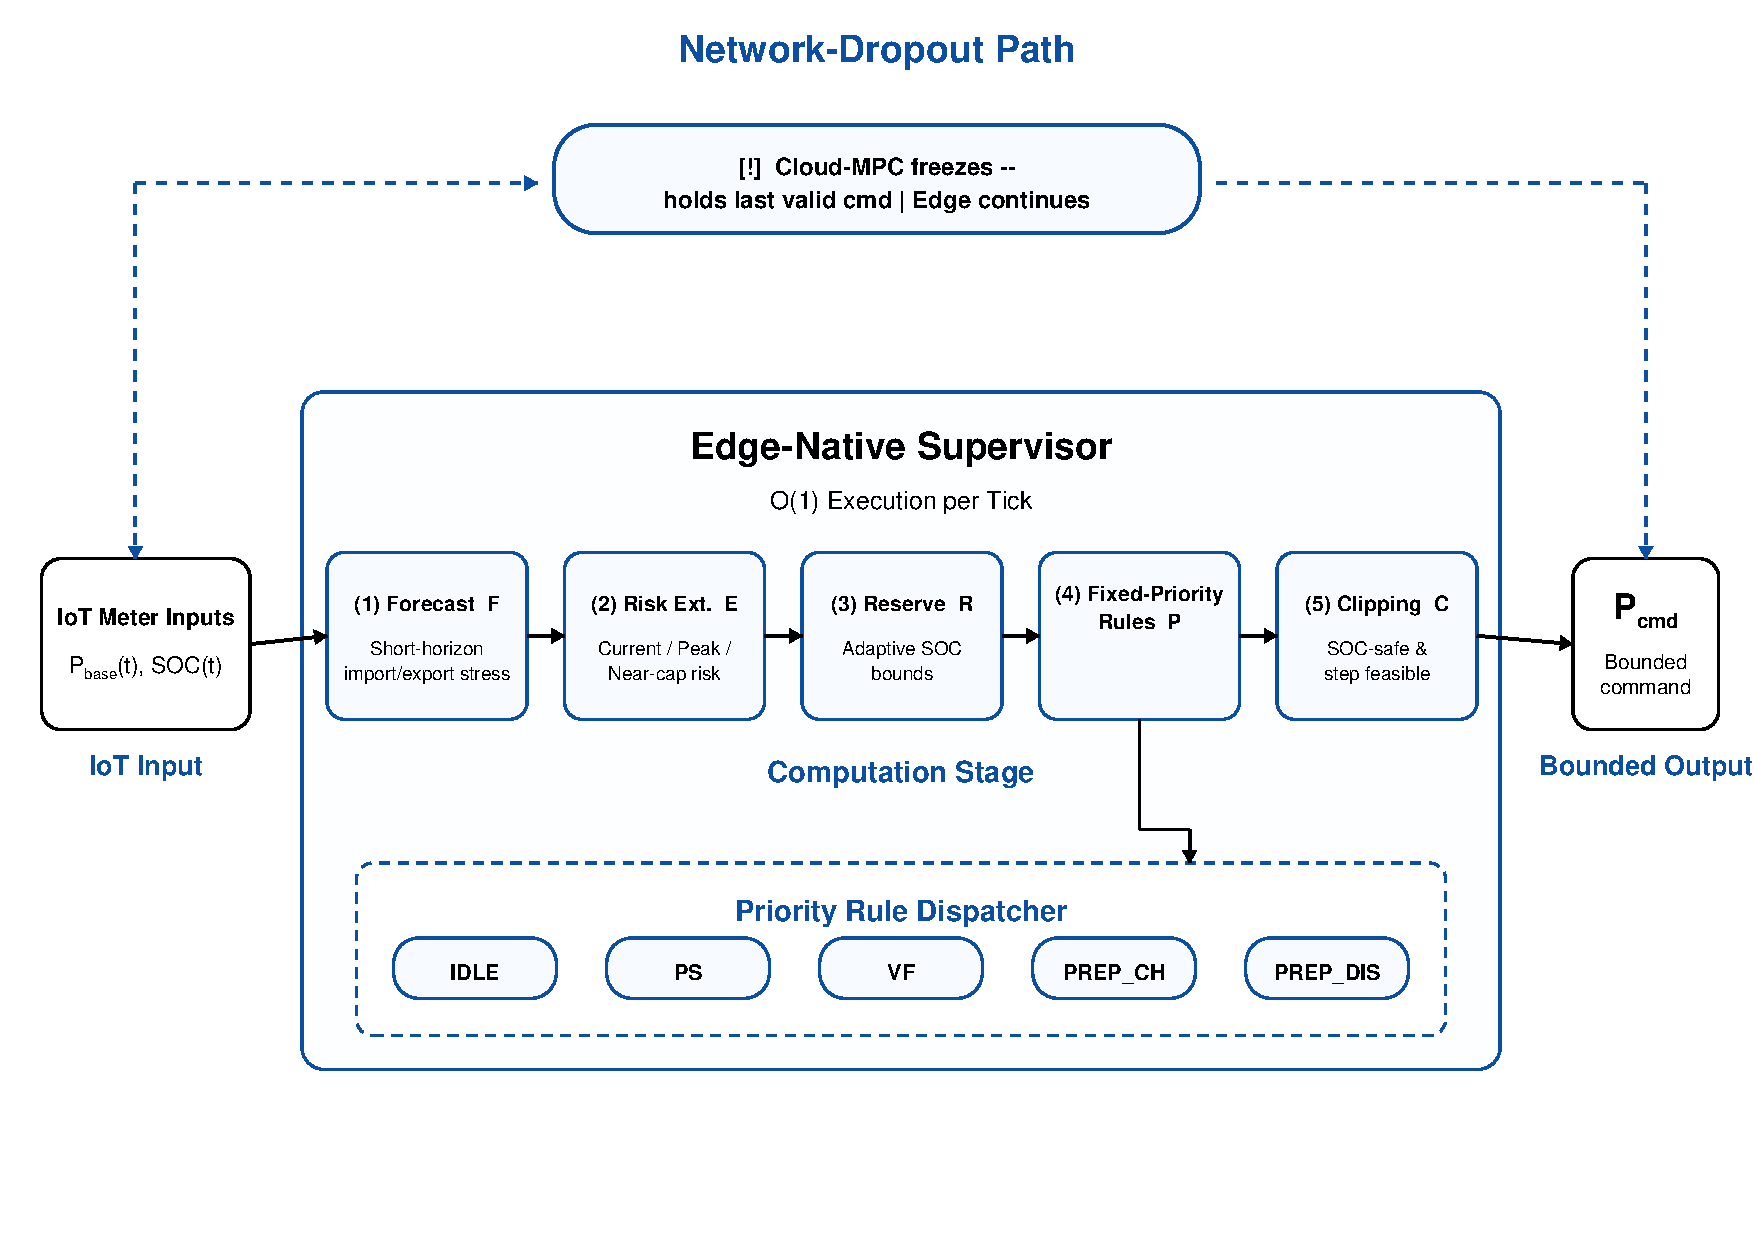
\includegraphics[width=\textwidth]{fig/runtime_path_diagram.pdf}
\caption{Runtime path of the released supervisory computing artifact. The software path is fixed in order: meter inputs feed a short-horizon forecast, risk extraction, reserve shaping, fixed-priority supervisory rules, and final clipping before a bounded command is emitted.}
\label{fig:runtime_path}
\end{figure}

The released controller does \emph{not} implement the earlier generic PS/VF/RG automaton. Instead, it logs one of five action labels
\[
\mathcal{M}=\{\texttt{PS},\texttt{VF},\texttt{PREP\_CH},\texttt{PREP\_DIS},\texttt{IDLE}\}
\]
and maintains a separate reserve indicator $r(t)\in\{\mathrm{LOW},\mathrm{MID},\mathrm{HIGH}\}$. The reserve indicator is used for logging and preparation logic; chatter suppression is implemented through short mode-specific action-hold rules rather than through a global dwell lock or emergency override branch.

\subsection{Adaptive reserve bands and reserve state}
The implemented controller starts from fixed soft reserve anchors
\[
s_{\mathrm{low}}^{(0)}=0.32,\qquad s_{\mathrm{high}}^{(0)}=0.62
\]
and adapts them according to predicted import/export stress:
\begin{align}
s_{\mathrm{low}}(t)
&= \clip\!\Big(
\clip\!\big(
s_{\mathrm{low}}^{(0)}
+ 0.10 \min(1,\tfrac{e_{\mathrm{imp,peak}}(t)}{\max(P_{\mathrm{imp,cap}}(t),1)}),
\ s_{\mathrm{low}}^{(0)},\ 0.54
\big) \notag\\
&\qquad
+ 0.03 \min(1,\tfrac{n_{\mathrm{imp}}(t)}{\Delta_{\mathrm{nc}}}),
\ s_{\mathrm{low}}^{(0)},\ 0.58
\Big), \\
s_{\mathrm{high}}(t)
&= \clip\!\Big(
\clip\!\big(
s_{\mathrm{high}}^{(0)}
- 0.06 \min(1,\tfrac{e_{\mathrm{exp,peak}}(t)}{\max(P_{\mathrm{exp,cap}}(t),1)}),
\ 0.50,\ s_{\mathrm{high}}^{(0)}
\big) \notag\\
&\qquad
- 0.03 \min(1,\tfrac{n_{\mathrm{exp}}(t)}{\Delta_{\mathrm{nc}}}),
\ 0.46,\ s_{\mathrm{high}}^{(0)}
\Big).
\end{align}
The logged reserve state is
\begin{equation}
r(t)=
\begin{cases}
\mathrm{LOW}, & \SOC(t)<s_{\mathrm{low}}(t),\\
\mathrm{HIGH}, & \SOC(t)>s_{\mathrm{high}}(t),\\
\mathrm{MID}, & \text{otherwise}.
\end{cases}
\end{equation}

\subsection{Priority decision rules}
At each tick, the controller evaluates rules in strict priority order. The first branch with a nonzero feasible request determines the provisional action label and desired command $\Pbatt^{\mathrm{des}}(t)$.

\paragraph{1. Immediate cap correction.}
If the current base sample already violates an import cap, the controller requests discharge:
\begin{equation}
\Pbatt^{\mathrm{des}}(t)=\min\!\Big(P_{\max}(t),\ e_{\mathrm{imp,now}}(t) + g_{\mathrm{la}}\max\big(0,e_{\mathrm{imp,peak}}(t)-e_{\mathrm{imp,now}}(t)\big)\Big),
\end{equation}
with $g_{\mathrm{la}}=0.01$, and logs mode \texttt{PS}. If the current base sample violates an export cap, it requests charge:
\begin{equation}
\Pbatt^{\mathrm{des}}(t)= -\min\!\Big(-P_{\min}(t),\ e_{\mathrm{exp,now}}(t) + g_{\mathrm{la}}\max\big(0,e_{\mathrm{exp,peak}}(t)-e_{\mathrm{exp,now}}(t)\big)\Big),
\end{equation}
and logs mode \texttt{VF}. These two branches have strict priority over all preparation behavior.

\paragraph{2. Low-power reserve preparation.}
If no current violation exists, the controller may pre-charge or pre-discharge so that future cap corrections can be delivered with lower stress. Define instantaneous slack margins
\begin{align}
\sigma_{\mathrm{imp}}(t) &= \max(0,\ P_{\mathrm{imp,cap}}(t)-\Pbase(t)),\\
\sigma_{\mathrm{exp}}(t) &= \max(0,\ P_{\mathrm{exp,cap}}(t)+\Pbase(t)).
\end{align}
The nominal preparation magnitudes are
\begin{align}
P_{\mathrm{prep,ch}}(t) &= -\min\!\big(4.0,\ 0.70\max(0,\sigma_{\mathrm{imp}}(t)-0.40)\big),\\
P_{\mathrm{prep,dis}}(t) &= \ \min\!\big(4.0,\ 0.70\max(0,\sigma_{\mathrm{exp}}(t)-0.40)\big).
\end{align}
A charge-preparation action (\texttt{PREP\_CH}) is entered when (i) forecasted or near-cap import risk exists, (ii) $\SOC(t)<s_{\mathrm{low}}(t)-0.02$, (iii) $\sigma_{\mathrm{imp}}(t)>1.5$~kW, or $>1.2$~kW in a near-cap window, and (iv) charging remains feasible ($P_{\min}(t)<0$). If the previous logged mode is already \texttt{PREP\_CH}, persistence is allowed under the softer conditions $\SOC(t)<s_{\mathrm{low}}(t)-0.01$ and $\sigma_{\mathrm{imp}}(t)>0.8$~kW. The discharge-preparation branch (\texttt{PREP\_DIS}) is defined symmetrically using export risk, $s_{\mathrm{high}}(t)$, and $\sigma_{\mathrm{exp}}(t)$.

\paragraph{3. Short action-hold rules.}
If neither direct correction nor preparation is triggered, the controller may still retain a decayed version of the previous command. When the previous mode is \texttt{PS} or \texttt{VF}, the action may persist for up to 3 ticks with decay factor $0.60$ if the next three forecast samples remain within 0.8~kW of the relevant cap. When the previous mode is \texttt{PREP\_CH} or \texttt{PREP\_DIS}, the action may persist for up to 5 ticks with the same decay factor while the corresponding reserve need and slack conditions remain active. This is the artifact's actual chatter-suppression mechanism.

\paragraph{4. Deadband and idle state.}
After the previous rules are evaluated, commands with magnitude below 0.25~kW are set to zero and the controller logs \texttt{IDLE}.

\subsection{Step-feasible command synthesis}
\label{subsec:cmd_synthesis}
Sequential application of saturation and step limits can create ambiguity (``saturate then limit'' vs ``limit then saturate''). To remove ordering ambiguity and guarantee physical feasibility, hard SOC/hardware bounds and the per-tick step constraint are enforced directly on the provisional request.

The parameter $\Rmax$ is defined as a \emph{per-tick command step limit} in kW:
\begin{equation}
|\Pcmd(t)-\Pcmd(t-1)| \le \Rmax.
\end{equation}
Let $\Delta t$ denote the control interval in minutes, given by $\Delta t = 60\Ts$ when $\Ts$ is in hours. The implied ramp-rate cap in kW/min equals $\Rmax/\Delta t$.

The symmetric step-feasibility window around the last command is
\begin{equation}
\mathcal{R}(t)=\left[\Pcmd(t-1)-\Rmax,\ \Pcmd(t-1)+\Rmax\right].
\end{equation}
The implementation then clips the provisional request directly to the feasible interval
\begin{align}
L(t) &= \max\!\big(P_{\min}(t),\ \Pcmd(t-1)-\Rmax\big),\\
U(t) &= \min\!\big(P_{\max}(t),\ \Pcmd(t-1)+\Rmax\big),\\
\Pcmd(t) &= \clip\!\big(\Pbatt^{\mathrm{des}}(t),L(t),U(t)\big).
\label{eq:pcmd_final}
\end{align}
This same hard-bound and step-limit clipping pattern is used throughout the rule-based baselines in the software artifact.

Under ideal tracking over $[t,t{+}1)$, $\Pbatt \approx \Pcmd(t)$ can be used in \eqref{eq:soc_update} to update $\SOC(t{+}1)$ from $\SOC(t)$.

% =========================================================
\begin{algorithm}[H]
\caption{FGCRP supervisory scheme: forecast-guided cap correction and reserve preparation}
\label{alg:plc}
\begin{algorithmic}[1]
\State \textbf{Inputs:} $\Pbase(t)$ and its trailing history, $\Pcmd(t-1)$, $\SOC(t)$, $u_{\mathrm{peak}}(t)$
\State \textbf{Key params:} $\alpha$, $w_f$, $K$, $\Dlim$, $\Rmax$, cap values, reserve-band constants, preparation constants
\State \textbf{State:} previous mode, dwell counter for repeated mode, previous command
\For{each tick $t$}
  \State Compute $\tau_{\mathrm{sat}}(t)=\clip(\MA^{\Delta}_{w_f}(\Pbase;t),-\Dlim,\Dlim)$
  \State Forecast $\widehat{\Pbase}(t+1..t+K)$ using \eqref{eq:forecast}
  \State Compute caps $P_{\mathrm{imp,cap}}(t),P_{\mathrm{exp,cap}}(t)$ via \eqref{eq:pimp_cap}--\eqref{eq:pexp_cap}
  \State Compute current, peak, and near-cap risk signals via \eqref{eq:eimp_now}--\eqref{eq:nexp}
  \State Update adaptive reserve bands $s_{\mathrm{low}}(t)$ and $s_{\mathrm{high}}(t)$
  \If{$e_{\mathrm{imp,now}}(t)>0$}
    \State request discharge with lookahead bonus; mode $\gets \texttt{PS}$
  \ElsIf{$e_{\mathrm{exp,now}}(t)>0$}
    \State request charge with lookahead bonus; mode $\gets \texttt{VF}$
  \ElsIf{charge-preparation entry/persistence conditions hold}
    \State request low-power charge; mode $\gets \texttt{PREP\_CH}$
  \ElsIf{discharge-preparation entry/persistence conditions hold}
    \State request low-power discharge; mode $\gets \texttt{PREP\_DIS}$
  \ElsIf{short action-hold conditions hold}
    \State request decayed previous command; keep previous action label
  \Else
    \State request zero power; mode $\gets \texttt{IDLE}$
  \EndIf
  \If{$|\Pbatt^{\mathrm{des}}(t)|<0.25$}
    \State set $\Pbatt^{\mathrm{des}}(t)\gets 0$ and mode $\gets \texttt{IDLE}$
  \EndIf
  \State Issue $\Pcmd(t)$ via hard-bound and step clipping \eqref{eq:pcmd_final}
  \State Update reserve indicator $r(t)$ from the adaptive reserve bands
  \State Update $\SOC(t{+}1)$ via \eqref{eq:soc_update}
\EndFor
\end{algorithmic}
\end{algorithm}

\begin{proposition}[FGCRP Execution and Feasibility Guarantees]
\label{prop:fgcrp}
Let $w_f\ge 1$ and $K\ge 1$ be fixed integer constants. Under the following assumptions:
\begin{enumerate}[label=\textbf{A\arabic*}]
  \item \textbf{(Bounded input)} $\Pbase(t)\in[P_{\min}^{\mathrm{site}}, P_{\max}^{\mathrm{site}}]$ for all $t$;
  \item \textbf{(Hardware limits)} $0 < P_{\mathrm{ch,max}}, P_{\mathrm{dis,max}} < \infty$ and $0 < \SOC_{\min} < \SOC_{\max} < 1$;
  \item \textbf{(Fixed parameters)} $w_f, K, \Rmax, \Dlim$ are compile-time constants independent of simulation length $N$;
\end{enumerate}
the FGCRP scheme (Algorithm~\ref{alg:plc}) guarantees, for every tick $t \ge 1$ and for all $S_{net}(t)\in\{0,1\}$:
\begin{enumerate}[label=\textbf{G\arabic*}]
  \item \textbf{(Constant-time execution)} The number of arithmetic operations per tick is bounded by $C_0(w_f + K)$ for a fixed constant $C_0$, i.e., $\mathcal{O}(w_f+K)=\mathcal{O}(1)$ under A3.
  \item \textbf{(Hard power feasibility)} $\Pcmd(t)\in[P_{\min}(t), P_{\max}(t)]$, where $P_{\min}(t), P_{\max}(t)$ are the SOC-implied and hardware-implied bounds from~\eqref{eq:hard_bounds}.
  \item \textbf{(Hard step feasibility)} $|\Pcmd(t) - \Pcmd(t-1)| \le \Rmax$.
\end{enumerate}
\end{proposition}
\begin{proof}[Proof sketch]
G1 follows from A3: the forecast loop~\eqref{eq:forecast} executes exactly $K$ scalar additions; the risk extraction~\eqref{eq:eimp_now}--\eqref{eq:nexp} and reserve-band update perform $\mathcal{O}(K)$ comparisons; the priority rule dispatcher (Algorithm~\ref{alg:plc}, the if-else block in the \textbf{For} loop) is a finite tree of depth~5 with no iteration; and the final clip~\eqref{eq:pcmd_final} is a single $\clip$ call. No data-dependent loops or solver calls appear anywhere in the path. G2 follows directly from the clip in~\eqref{eq:pcmd_final}: $\Pcmd(t)=\clip(\Pbatt^{\mathrm{des}}(t), L(t), U(t))$ where $L(t)\ge P_{\min}(t)$ and $U(t)\le P_{\max}(t)$ by construction. G3 holds in the non-degenerate case where $P_{\max}(t)\ge\Pcmd(t-1)-\Rmax$ and $P_{\min}(t)\le\Pcmd(t-1)+\Rmax$; when the SOC-implied window is narrower than the step limit (e.g., near SOC depletion), the clip forces $\Pcmd(t)=P_{\max}(t)$ or $P_{\min}(t)$, constituting a forced override in which SOC safety takes precedence over the ramp constraint---a standard priority ordering in BESS protection logic. These guarantees hold for all $t$ regardless of $S_{net}(t)$, since the execution path contains no network call.
\end{proof}

\textit{Remark:} Cloud-MPC cannot provide G1--G3 unconditionally: during a network dropout ($S_{net}(t)=0$), the solver is unreachable, so neither the optimal action nor feasibility can be guaranteed without a local fallback. The FGCRP scheme is, by design, its own local fallback.

\begin{table}[H]
\centering
\caption{Fixed-memory summary of the released controller at the default 1-minute setting.}
\label{tab:fixed_memory}
\footnotesize
\setlength{\tabcolsep}{4pt}
\begin{tabularx}{\textwidth}{@{} l c Y @{}}
\toprule
Component & Count & Role in the bounded-time path \\
\midrule
Base-history ring buffer & $w_f + 1 = 6$ samples & Reproduces the moving-average and trend terms used by the ultra-light forecast. \\
Forecast scratch buffer & $K = 10$ samples & Stores the short-horizon forecast values used by risk extraction and reserve shaping. \\
Previous command & 1 scalar & Supports direct step clipping and short action-hold decay. \\
Previous mode label & 1 enum & Records the last action family (\texttt{PS}, \texttt{VF}, \texttt{PREP\_CH}, \texttt{PREP\_DIS}, \texttt{IDLE}). \\
Reserve label & 1 enum & Records the current reserve region (\texttt{LOW}, \texttt{MID}, \texttt{HIGH}). \\
Dwell counter & 1 integer & Limits the hold duration of repeated cap-fix or preparation actions. \\
\bottomrule
\end{tabularx}
\end{table}

% =========================================================
\subsection{Computational Complexity and Real-Time Feasibility}
With fixed short horizons ($w_f=5$, $K=10$ in the reported benchmark), the studied controller performs only bounded arithmetic on trailing windows plus a constant number of comparisons and clips. The software implementation therefore scales as $\mathcal{O}(w_f+K)$ per tick with no iterative solve or matrix factorization in the proposed policy itself. Since $w_f$ and $K$ are fixed configuration constants independent of the simulation horizon $N$, this is equivalently $\mathcal{O}(1)$ per tick---the notation used throughout the abstract and highlights. This is the structural reason the measured runtime remains in the sub-millisecond range, whereas the optimization baseline is orders of magnitude slower.

The fixed-memory interpretation should be read directly from \Cref{tab:fixed_memory}: beyond two short arrays of length $w_f+1$ and $K$, the controller retains only four persistent values (previous command, previous mode label, reserve label, dwell counter). When scan time is shortened in the supplementary extension tests, these array lengths scale deterministically with the chosen interval to keep the physical look-back and look-ahead windows approximately comparable.

\subsection{Deployment Mapping and Claim Boundary}
The manuscript uses the term \emph{PLC/SCADA-executable} in an architectural, deployment-oriented sense, not as a claim of vendor-certified execution on a specific PLC family. The compatibility argument rests on the implemented I/O structure, fixed memory footprint, bounded arithmetic path, and software-measured timing envelope of the studied scheme.

\begin{table}[H]
\centering
\caption{Implementation features supporting the architectural PLC/SCADA-executability claim.}
\label{tab:deployment}
\footnotesize
\setlength{\tabcolsep}{3pt}
\resizebox{\textwidth}{!}{%
\begin{tabular}{@{} l l l @{}}
\toprule
Aspect & Implemented controller property & Deployment interpretation \\
\midrule
External inputs & $\Pbase(t)$ (or equivalent load/PV/wind tags), $\SOC(t)$, peak-flag schedule & SCADA-readable scalar tags \\
Persistent state & previous command, previous mode label, reserve label, dwell counter & four persistent scalars/enums only \\
Short memory & $w_f+1=6$ recent base samples suffice to reproduce the forecast logic & small ring buffer or shift-register realization \\
Arithmetic pattern & comparisons, min/max, clipping, and a 10-step forecast loop & standard IEC 61131 structured-text / function-block operations \\
Unavailable in the proposed path & no matrix factorization, nonlinear program, or iterative numerical solver & no solver dependency in the rule engine \\
Software timing evidence & Proposed: 0.290--0.347 ms/tick across 6h/12h/24h runs; MPC: 813--1179 ms/tick & relative real-time margin on the reference workstation \\
\bottomrule
\end{tabular}}
\end{table}

Table~\ref{tab:deployment} makes the deployment claim precise. The released rule engine can be mapped to a small number of scalar tags and persistent variables, and its forecast can be reproduced with a ring buffer of six recent base samples rather than with unbounded history. Equally important, the controller uses only fixed-depth arithmetic and branching; there is no optimization call, matrix inversion, or data-dependent iteration count in the proposed execution path. These are the properties that support the compatibility claim.

The boundary of the claim is equally important. The reported timing values are collected from the Python reference implementation on a general-purpose workstation via \texttt{time.perf\_counter()}, so they should be interpreted as software evidence of bounded complexity and as a relative comparison against \texttt{MPC\_ref}, not as a hardware certification for a specific PLC family. This distinction from optimization-centric EMS is deliberate: recent microgrid studies continue to place MPC inside the online loop \cite{li2025twotimescale}. Bayesian supervisory optimization remains another heavier alternative \cite{brown2026bayesian}. By contrast, the present claim is specifically about a solver-free supervisory computing path that remains auditable at scan-time granularity and suitable for edge or PLC-style execution. Hardware-in-the-loop and vendor-specific PLC deployment remain future validation tasks, and the manuscript does not claim that such validation has already been completed.

Safety handling is also intentionally narrow. The released controller guarantees feasible commands only through the hard clipping logic of \eqref{eq:pcmd_final}; it does not contain a native missing-sample branch, delay compensator, or stale-forecast recovery mode. Accordingly, the supplementary robustness experiment reported later inserts an \emph{external} hold-last-sample preprocessing wrapper ahead of the controller and should be interpreted as a channel-sensitivity bound, not as evidence that the controller already implements built-in fault-tolerant estimation.

% =========================================================
\section{Software Platform and Evaluation Protocol} \label{sec:experiments}
\subsection{Test configuration}
Experiments target a grid-connected PV--wind microgrid with a lithium-ion BESS as the application setting for the proposed supervisory computing artifact.
Signals are sampled at minute-level cadence to align with real-time PLC/SCADA supervisory loops and to expose whether the online decision path remains lightweight relative to the control interval.
The BESS is constrained by:
(i) charge/discharge power limits ($P_{\mathrm{ch,max}}$, $P_{\mathrm{dis,max}}$),
(ii) SOC bounds (default $\SOC_{\min}=0.2$ (20\%), $\SOC_{\max}=0.8$ (80\%), $\SOC_{\mathrm{init}}=0.5$), and
(iii) per-tick command step limit $\Rmax=20$~kW (enforced on $\Pcmd$ by \eqref{eq:pcmd_final}). The reported software defaults further use $P_{\mathrm{ch,max}}=P_{\mathrm{dis,max}}=50$~kW, $E_{\mathrm{nom}}=100$~kWh, $\eta_{\mathrm{ch}}=\eta_{\mathrm{dis}}=0.95$, and symmetric 40~kW import/export caps.

\subsection{Software realization and result provenance}
The reported study follows the exact execution order of the released application: a seed-controlled synthetic profile is generated, the chosen controller is executed inside a discrete-time simulator using the directly available $\Pbase$ history, per-scenario-day metrics are computed from the resulting trajectories, and final comparison tables/figures are exported from those aggregated records. The manuscript therefore mirrors the software pipeline rather than a separate analytical prototype.

The primary manuscript tables and figures correspond to the fixed reproducibility artifact \texttt{outputs\_24h\_core\_eval}. Its manifest specifies a 24-hour benchmark with scenario families \texttt{mixed}, \texttt{cloud\_edge}, \texttt{wind\_gust}, and \texttt{load\_step}; seeds 0 and 1; and the controller set \texttt{Proposed}, \texttt{NC}, \texttt{GR}, \texttt{RS}, \texttt{FBRL}, and \texttt{MPC\_ref}. This explicit provenance is important because the repository also contains broader sweeps, oracle diagnostics, and publication-audit utilities that are not part of the manuscript's primary quantitative claim.

\subsection{Data sources and synthetic profile generation}
\label{subsec:synth_gen}
Evaluation profiles must capture fast cloud-edge PV ramps, sustained wind intermittency, and step-like load changes. To emulate these extremes concurrently, the software generates minute-level synthetic stress-test profiles as $\Pbase(t)=\Pload(t)-(\Ppv(t)+\Pwind(t))$. The load process uses a daily sinusoid with base 48~kW, amplitude 12~kW, Gaussian noise of 2.5~kW, and slowly decaying step events drawn with probability 0.30/h from the interval $[-10,14]$~kW; the \texttt{load\_step} scenario doubles this step probability. PV uses a daylight half-sine with peak 45~kW, multiplied by a transmittance state perturbed by cloud events (base probability 1.2/h, target transmittance 0.2--0.9, duration 1--3 min, plus 0.6~kW measurement noise). Wind is generated by an AR(1)-like baseline with coefficient 0.85, base level 14~kW, Gaussian noise 2.5~kW, and positive gust injections (base probability 0.7/h, amplitude 8--20~kW). The four scenario families used in the primary benchmark are \texttt{mixed}, \texttt{cloud\_edge}, \texttt{wind\_gust}, and \texttt{load\_step}; all random draws are seeded and results are aggregated over two seeds.

\subsection{Baselines and reference bounds}
\label{subsec:baselines}

The baseline set includes simple comparators (RS/GR/NC) and two stronger references: a filter-based industrial shaper and an optimization-based receding-horizon controller. Perfect-preview and global oracle variants are available in the reproducibility package as diagnostic references, but they are excluded from the main manuscript tables.

To ensure a fair comparison, all controllers share identical SOC/power limits, efficiencies, and the same 40~kW PCC caps. The rule-based baselines all enforce hard bounds and the same per-tick step clip after forming a desired command. The optimization baseline enforces the same step constraint directly inside the QP. Recent microgrid EMS work continues to use optimization-based supervisory controllers as strong performance references \cite{li2025twotimescale}. Bayesian supervisory tuning provides another optimization-rich reference family \cite{brown2026bayesian}. Learning-based safe dispatch offers a further comparison class \cite{yang2025shieldeddrl}. Accordingly, the benchmark set combines simple rule baselines with one explicit MPC-QP reference, while keeping the studied controller solver-free.

\begin{itemize}
\item \textbf{No control (NC):} Battery disabled with $\Pcmd(t)\equiv 0$ for all $t$, hence $\Pbatt(t)=0$ and $\Pgrid(t)=\Pbase(t)$.

\item \textbf{Greedy rule-based (GR):} Forecast-free threshold policy with SOC triggers.\par
If $\SOC(t)\le \SOC_{\min}+\delta_s$, the controller requests the maximum feasible charge. If $\SOC(t)\ge \SOC_{\max}-\delta_s$, it requests the maximum feasible discharge. Otherwise, it only reacts to the current cap violation and stays idle.

\item \textbf{Reactive smoothing (RS):}\par
Moving-average smoother.\par
No forecast-based anticipation is used. A trailing average of the recent base history defines the reference. The desired battery request is
\[
\Pbatt^{\mathrm{des}}(t)=\Pbase(t)-\overline{\Pbase}_{w_f}(t),
\]
with no reserve logic.

\item \textbf{Filter-based reference shaping (FBRL) (state-of-practice):}
An industrial approach is emulated by applying a low-pass filter to the base signal, consistent with earlier ramp-control studies \cite{marcos2014}. Related storage-assisted shaping strategies have also been reported \cite{damico2022}. An exponentially smoothed estimate $\widetilde{\Pref}(t)$ is computed using parameter $\beta=2/(w_{\mathrm{ema}}+1)$, and bounded to form $\Pref^{\mathrm{cap}}(t)=\clip\!\big(\widetilde{\Pref}(t),\ -P_{\mathrm{exp,cap}}(t),\ P_{\mathrm{imp,cap}}(t)\big)$. The desired battery request directly follows as $\Pbatt^{\mathrm{des}}(t)=\Pbase(t)-\Pref^{\mathrm{cap}}(t)$.

\item \textbf{Linear MPC-QP (benchmark, not PLC-targeted):}
A constrained receding-horizon controller solving a quadratic program over horizon $K=10$ using the same forecast model as the rule-based controller. The decision variable is the command sequence $\{u_k\}_{k=0}^{K-1}$ with $u_{-1}\triangleq \Pcmd(t-1)$. The implemented objective is
\begin{equation}
\begin{aligned}
\min_{\{u_k\}} \quad
& \rho_{\mathrm{imp}}\sum_{k=0}^{K-1}\big[\max(0,\widehat{\Pbase}(t+k)-u_k-P_{\mathrm{imp,cap}}(t+k))\big]^2 \\
&+ \rho_{\mathrm{exp}}\sum_{k=0}^{K-1}\big[\max(0,-\widehat{\Pbase}(t+k)+u_k-P_{\mathrm{exp,cap}}(t+k))\big]^2 \\
&+ \lambda \sum_{k=0}^{K-1} u_k^2 \\
&+ \mu \Big((u_0-u_{-1})^2 + \sum_{k=1}^{K-1}(u_k-u_{k-1})^2\Big) \\
&+ \nu \sum_{k=0}^{K-1}(\SOC_k-\SOC_{\mathrm{mid}})^2 ,
\end{aligned}
\label{eq:mpc_qp_obj}
\end{equation}
subject to hard command bounds, nonlinear SOC constraints using the same asymmetric charge/discharge efficiencies as the simulator, and explicit step constraints $|u_k-u_{k-1}|\le \Rmax$. Only the first action $u_0$ is applied. In the released simulator, if future peak flags are not explicitly supplied, the current peak flag is repeated across the optimization horizon; in the primary benchmark this distinction is immaterial because all import/export caps are fixed at 40~kW. The primary benchmark uses the fixed weight tuple $(\lambda,\mu,\nu)=(10^{-2},10^{-2},10^{-3})$ and $\rho_{\mathrm{imp}}=\rho_{\mathrm{exp}}=10^4$, solved with SciPy \texttt{trust-constr}.\par \textit{Fairness note:} \texttt{MPC\_ref} is used as one transparent, reproducible optimization reference implemented inside the released codebase. It is not presented as an exhaustive upper bound on all possible MPC designs or tuning choices.

\item \textbf{Oracle references (artifact-only):}\par
The codebase also includes perfect-preview receding-horizon sweeps and a full-horizon global oracle in \texttt{optimization\_refs.py}. They are retained for artifact-level diagnostics and excluded from the manuscript's primary comparison table.
\end{itemize}

For ultra-light comparisons, the released artifact also exposes a no-forecast ablation variant (\texttt{A1}) in addition to GR and RS. This variant is not elevated to the main comparison table because it is derived from the proposed controller family rather than defined as an independent literature baseline, but it remains useful when the manuscript later separates compute cost from application behavior in the supplementary extension analysis.

\subsection{Metrics}
Grid-facing and battery-usage/sustainability metrics include:
\begin{itemize}
\item \textbf{95th-percentile ramp rate at PCC:} Let $\Delta t$ denote the control interval in minutes (with $\Delta t=60\Ts$ when $\Ts$ is in hours). Define the per-tick step $\Delta P_{\mathrm{grid}}(t)=|\Pgrid(t)-\Pgrid(t-1)|$ (kW) and the ramp rate
\begin{equation}
r_{\mathrm{grid}}(t)=\frac{\Delta P_{\mathrm{grid}}(t)}{\Delta t}\quad \text{(kW/min)}.
\end{equation}
The 95th percentile of $r_{\mathrm{grid}}(t)$ is reported.

\item \textbf{Cap-violation exposure:}
import-cap violation indicator $v_{\mathrm{imp}}(t)=\mathbf{1}\{\Pgrid(t)>P_{\mathrm{imp,cap}}(t)\}$ and
export-cap violation indicator $v_{\mathrm{exp}}(t)=\mathbf{1}\{-\Pgrid(t)>P_{\mathrm{exp,cap}}(t)\}$.
Report the percentage of ticks with $v_{\mathrm{imp}}(t)=1$ and $v_{\mathrm{exp}}(t)=1$.

\item \textbf{SOC band residency:} fraction of time $\SOC(t)\in[\SOC_{\min},\SOC_{\max}]$.

\item \textbf{Throughput:} $\sum_t |\Pcmd(t)|\,\Ts$ (kWh).

\item \textbf{Equivalent full cycles (EFC):}
\begin{equation}
\EFC \approx \frac{\sum_t |\Pcmd(t)|\,\Ts}{2E_{\mathrm{nom}}}.
\label{eq:efc}
\end{equation}
\textit{Remark:} This standard EFC metric serves as a proxy for total energy throughput and thermal stress \cite{hoke2014accounting}.

\item \textbf{Rainflow-based cycle counting and micro-cycling indicators:}
To capture mechanical fatigue and irregular cycling often missed by throughput metrics, cycle counting is performed offline on the logged SOC trajectory using rainflow analysis. Rainflow-based battery-stress reporting is standard in storage studies \cite{gundogdu2018}. Cycle-depth-oriented assessment has also been used in related work \cite{soto2022}. Data-driven battery analysis pipelines frequently rely on comparable cycle decomposition \cite{attia2022}. SOC-safe battery-control studies further motivate depth-aware cycle accounting \cite{he2018convex}. Rainflow counting yields a set of cycle elements indexed by $j=1,\dots,J$, each with depth $\Delta \SOC_j\in(0,1]$ and a count weight $c_j\in\{0.5,1\}$. A count-weighted \emph{rainflow cycle-depth sum} (dimensionless), denoted by $\EFCrf$, is defined as
\begin{equation}
\EFCrf \triangleq \sum_{j=1}^{J} c_j\,\Delta \SOC_j .
\label{eq:efc_rf}
\end{equation}
\textit{Remark:} If a full-cycle equivalent comparable to energy-based $\EFC$ in \eqref{eq:efc} is required, use $\EFCrf^{\mathrm{full}} \triangleq \tfrac{1}{2}\EFCrf$.

The count-weighted micro-cycle indicator is defined as
\begin{equation}
\Nmicro(\dmc) \triangleq \sum_{j=1}^{J} c_j\,\mathbf{1}\{\Delta \SOC_j \le \dmc\},
\label{eq:nmicro}
\end{equation}
where $\dmc$ is the micro-cycle depth threshold (e.g., $\dmc\in[0.01,0.05]$ SOC).

\item \textbf{Chemistry-calibrated cycling sustainability indicator (LiFePO$_4$):}
To complement proxy-only stress reporting, a direct modeled cycling-sustainability indicator is also computed using a room-temperature LiFePO$_4$ cycle-life fit \cite{wang2011lfp}. An operational life-loss mapping is then applied to the realized dispatch intervals \cite{yan2018lifeloss}. Let $\SOC_j^{-}$ and $\SOC_j^{+}$ denote the lower and upper SOC bounds of rainflow element $j$, with $\SOC_j^{-}\le \SOC_j^{+}$ and count weight $c_j\in\{0.5,1\}$. Following the operational life-loss formulation of \cite{yan2018lifeloss}, the cycle-life curve for repeated cycling between $\SOC_i$ and $100\%$ SOC is written as
\begin{equation}
C(\SOC_i)=28270\,e^{-2.401(1-\SOC_i)} + 2.214\,e^{5.901(1-\SOC_i)},
\label{eq:lfp_cycle_life}
\end{equation}
where $C(\SOC_i)$ is the number of cycles to the reference end-of-life threshold under the fitted LiFePO$_4$ conditions. Each rainflow element contributes a modeled fractional cycling impact
\begin{equation}
x_j = c_j \left| \frac{1}{2\,C(\SOC_j^-)} - \frac{1}{2\,C(\SOC_j^+)} \right|,
\label{eq:lfp_cycle_loss_element}
\end{equation}
and the horizon-level modeled cycling indicator is reported as
\begin{equation}
X_{\mathrm{LFP}}^{\mathrm{cyc}} = 100 \sum_{j=1}^{J} x_j \qquad (\%).
\label{eq:lfp_cycle_loss}
\end{equation}
\textit{Remark:} Unlike EFC or IDOD, $X_{\mathrm{LFP}}^{\mathrm{cyc}}$ is not a generic proxy; it maps the realized SOC intervals through a chemistry-specific cycle-life curve. In the manuscript it is treated as downstream, application-facing sustainability evidence rather than as a core novelty claim. It remains a modeled estimate rather than field-measured capacity fade.

\item \textbf{Action switching rate:} Let $m(t)\in\mathcal{M}$ be the logged action label sequence over $N$ ticks, where $\mathcal{M}=\{\texttt{PS},\texttt{VF},\texttt{PREP\_CH},\texttt{PREP\_DIS},\texttt{IDLE}\}$ for the studied controller and the analogous logged labels for the other baselines. Define
\begin{equation}
N_{\mathrm{flip}}=\sum_{t=2}^{N}\mathbf{1}\{m(t)\neq m(t-1)\}.
\label{eq:nflip}
\end{equation}
With $\Ts$ in hours, the horizon is $H=N\Ts$ hours. Report
\begin{equation}
\text{flip/hour}=\frac{N_{\mathrm{flip}}}{H},\qquad
\text{flip/day}=\frac{N_{\mathrm{flip}}}{H/24}.
\label{eq:flip_rates}
\end{equation}

\item \textbf{Measured compute time:} the simulator measures per-tick wall-clock execution time using \texttt{time.perf\_counter()} around each controller step and reports mean/median/P95 CPU time in milliseconds. This is an actual runtime measurement for the released software, not a normalized proxy.

\item \textbf{Resilience Score ($R_{score}$) and Compliance Degradation Index ($CDI$):}
The Resilience Score quantifies the ability of a controller to maintain grid-cap compliance during offline events ($S_{net}(t) = 0$). It is defined as the complement of the cap-violation fraction restricted to offline ticks:
\begin{equation}
R_{score} = 100 \times \left(1 - \frac{\sum_{t \in T_{offline}} (v_{\mathrm{imp}}(t) \lor v_{\mathrm{exp}}(t))}{\max(|T_{offline}|,1)}\right)
\label{eq:resilience_score}
\end{equation}
where $T_{offline} = \{t \mid S_{net}(t) = 0\}$. A score of 100\% means no cap violation occurs during any disconnected tick.

Note on interpretation: for a controller whose cap-violation rate is structurally zero (e.g., the proposed Edge heuristic), $R_{score}=100\%$ by design and is not informative in isolation. The complementary \emph{Compliance Degradation Index} (CDI) is therefore also reported, defined as the difference in cap-violation rate between offline and online ticks:
\begin{equation}
CDI = v_{\mathrm{cap}}^{\mathrm{offline}} - v_{\mathrm{cap}}^{\mathrm{online}},
\quad v_{\mathrm{cap}}^{\star} = \frac{\sum_{t\in T_{\star}} (v_{\mathrm{imp}}(t)\lor v_{\mathrm{exp}}(t))}{\max(|T_{\star}|,1)}
\label{eq:cdi}
\end{equation}
where $T_{\mathrm{online}}=\{t\mid S_{net}(t)=1\}$. A positive CDI reveals structural vulnerability: the controller performs worse during offline periods. For an Edge-native controller, $CDI=0$ by construction; for a Cloud-dependent controller with HLA fallback, $CDI > 0$ in scenarios where the held command diverges from the cap boundary.
\end{itemize}

\begin{table}[H]
\centering
\caption{Implemented default parameters used in the primary benchmark and in the studied supervisory scheme.}
\label{tab:params}
\small
\setlength{\tabcolsep}{4pt}
\renewcommand{\arraystretch}{1.06}
\begin{tabularx}{\textwidth}{@{}>{\raggedright\arraybackslash}p{0.18\textwidth} Y >{\raggedright\arraybackslash}p{0.22\textwidth}@{}}
\toprule
Block & Setting & Value \\
\midrule
Plant/BESS & $\Ts$, $P_{\mathrm{ch,max}}$, $P_{\mathrm{dis,max}}$, $E_{\mathrm{nom}}$ & 1 min; 50/50 kW; 100 kWh \\
Plant/BESS & $\eta_{\mathrm{ch}}$, $\eta_{\mathrm{dis}}$, $\SOC_{\min}$, $\SOC_{\max}$, $\SOC_{\mathrm{init}}$ & 0.95/0.95; 0.20/0.80/0.50 \\
Grid caps & $P_{\mathrm{imp,contr}}$, $P_{\mathrm{exp,phys}}$, peak/off-peak caps, $\Delta_{\mathrm{imp}}$, $\Delta_{\mathrm{exp}}$ & 40/40 kW; 40/40 kW; 0/0 \\
Forecast & $\alpha$, $w_f$, $K$, $\Dlim$ & 0.30; 5; 10; 8.0 kW/tick \\
Rule logic & $\Rmax$, $\delta_s$, $w_{\mathrm{ema}}$, $\dmc$ & 20.0 kW/tick; 0.02; 7; 0.02 \\
Proposed & soft reserve anchors $s_{\mathrm{low}}^{(0)}$, $s_{\mathrm{high}}^{(0)}$ & 0.32 / 0.62 \\
Proposed & lookahead gain, prep power cap, min useful command & 0.01; 4.0 kW; 0.25 kW \\
Proposed & reserve enter/exit margins & 0.02 / 0.01 \\
Proposed & cap-fix hold ticks / prep hold ticks / hold decay & 3 / 5 / 0.60 \\
Proposed & near-cap buffer / near-cap margin / SOC boost & 1.5 kW / 0.8 kW / 0.03 \\
Proposed & prep slack gain / offset / near-cap prep slack & 0.70 / 0.40 / 1.2 kW \\
Benchmark & scenario families and seeds & mixed, cloud\_edge, wind\_gust, load\_step; seeds 0 and 1 \\
Benchmark & horizon length and peak-flag schedule & 24 h; 17:00--22:00 \\
MPC\_ref & $(\lambda,\mu,\nu)$ and $(\rho_{\mathrm{imp}},\rho_{\mathrm{exp}})$ & $(10^{-2},10^{-2},10^{-3})$ and $(10^4,10^4)$ \\
\bottomrule
\end{tabularx}
\end{table}

\subsection*{Parameter provenance, tuning protocol, and sensitivity}
Table~\ref{tab:params} should not be read as a list of equally free tuning knobs. The plant ratings, efficiencies, SOC bounds, PCC caps, and peak-period schedule are benchmark definitions and were never searched. The ablation switches A1--A6 are also not tuning parameters; they are causal mechanism removals used later to test whether forecast, reserve persistence, short action-hold, and reserve-correction logic materially matter. The actual search space was intentionally narrow and restricted to four aggressiveness parameters that most directly shape behavior: the lower soft-reserve anchor, the preparation power cap, the lookahead gain, and the minimum useful command threshold. In the released code these correspond to \texttt{base\_soft\_low}, \texttt{prep\_power\_cap\_kw}, \texttt{lookahead\_gain}, and \texttt{min\_useful\_cmd\_kw}.

To avoid selecting these values from the same single benchmark that is later used for the headline comparison, a separate parameter audit was run on the union of all currently available post-fix, non-smoke datasets: the 6-hour compact tier, the 12-hour medium tier, and the 24-hour core tier, for a total of 20 scenario-seed units. The canonical split trains on all seed-0 units and evaluates on all seed-1 units across the three tiers. Five additional repeated splits reverse the seed split, swap short/medium tiers versus the 24-hour tier, and swap the milder scenario families (\texttt{mixed}, \texttt{cloud\_edge}) versus the more severe ones (\texttt{wind\_gust}, \texttt{load\_step}). Candidate quality is scored only against GR using the same metric family emphasized in the manuscript. This choice is used to keep the released controller near the conservative low-stress region represented by GR; it is not presented as evidence that GR is the only relevant benchmark or that the selected point is globally optimal. The score is
\begin{equation}
J = \Delta r_{95} + 2\,\Delta v_{\mathrm{cap}} + 0.25\,\Delta E_{\mathrm{thru}} + 75\,\Delta \mathrm{IDOD} + 0.05\,\Delta N_{\mathrm{flip/day}},
\label{eq:param_score}
\end{equation}
where $\Delta$ denotes candidate-minus-GR mean on the relevant split and lower values are better. This scoring intentionally weights cap-violation reduction and deeper cycling more strongly than very small throughput differences, but it should be read as a stabilization device for the released setting rather than as a universal tuning objective.

The resulting search audit does \emph{not} support a sharp single-point optimum. The best candidate over the six repeated splits is $(0.32,\ 3.0,\ 0.01,\ 0.25)$ with mean hold score 0.0576, but the released default used throughout the manuscript, $(0.32,\ 4.0,\ 0.01,\ 0.25)$, follows immediately with mean hold score 0.0595 and the same zero mean hold-out cap delta. A third nearby setting, $(0.32,\ 5.0,\ 0.01,\ 0.25)$, yields 0.0622. The manuscript deliberately retains the released default rather than replacing it with the numerically best point after the audit, precisely to avoid presenting a last-minute benchmark-specific retune as if it were essential. Thus, the published controller should be interpreted as lying on a flat hold-out performance plateau rather than as the result of aggressive single-benchmark fitting. The audit therefore supports parameter stability of the released variant, not universal parameter optimality.

\begin{table}[H]
\centering
\caption{Grouped sensitivity of the four searched aggressiveness parameters over the 20-profile cross-tier parameter audit. Entries report mean hold-out score versus GR (lower is better) and mean hold-out cap-violation delta versus GR.}
\label{tab:param_search_sensitivity}
\footnotesize
\setlength{\tabcolsep}{4pt}
\resizebox{\textwidth}{!}{%
\begin{tabular}{@{} l l l l @{}}
\toprule
Search parameter & Scanned values & Mean hold score vs GR & Mean hold cap delta vs GR \\
\midrule
Lower soft-reserve anchor & 0.32 / 0.34 / 0.36 / 0.38 & 0.069 / 0.206 / 0.424 / 0.524 & 0.0000 / 0.0000 / 0.0101 / 0.0081 \\
Lookahead gain & 0.01 / 0.02 / 0.04 & 0.105 / 0.234 / 0.489 & 0.0000 / 0.0020 / 0.0101 \\
Preparation power cap (kW) & 3 / 4 / 5 & 0.129 / 0.178 / 0.347 & 0.0000 / 0.0012 / 0.0068 \\
Minimum useful command (kW) & 0.25 / 0.50 & 0.123 / 0.336 & 0.0000 / 0.0057 \\
\bottomrule
\end{tabular}}
\end{table}

Table~\ref{tab:param_search_sensitivity} shows that the selected region is not arbitrary. Lower reserve anchors above 0.34 markedly worsen the hold-out score, and the 0.36/0.38 settings begin to introduce positive mean cap-violation deltas relative to GR. Likewise, larger lookahead gains and larger minimum-command thresholds degrade hold-out behavior instead of improving it. The preparation power cap exhibits a shallow optimum: 3--4~kW form the stable plateau, while 5~kW becomes clearly more aggressive. This is exactly the opposite of a hidden overfit narrative: the chosen default is a conservative interior point of the low-score plateau, not a fragile extreme.

\begin{figure}[!htbp]
\centering
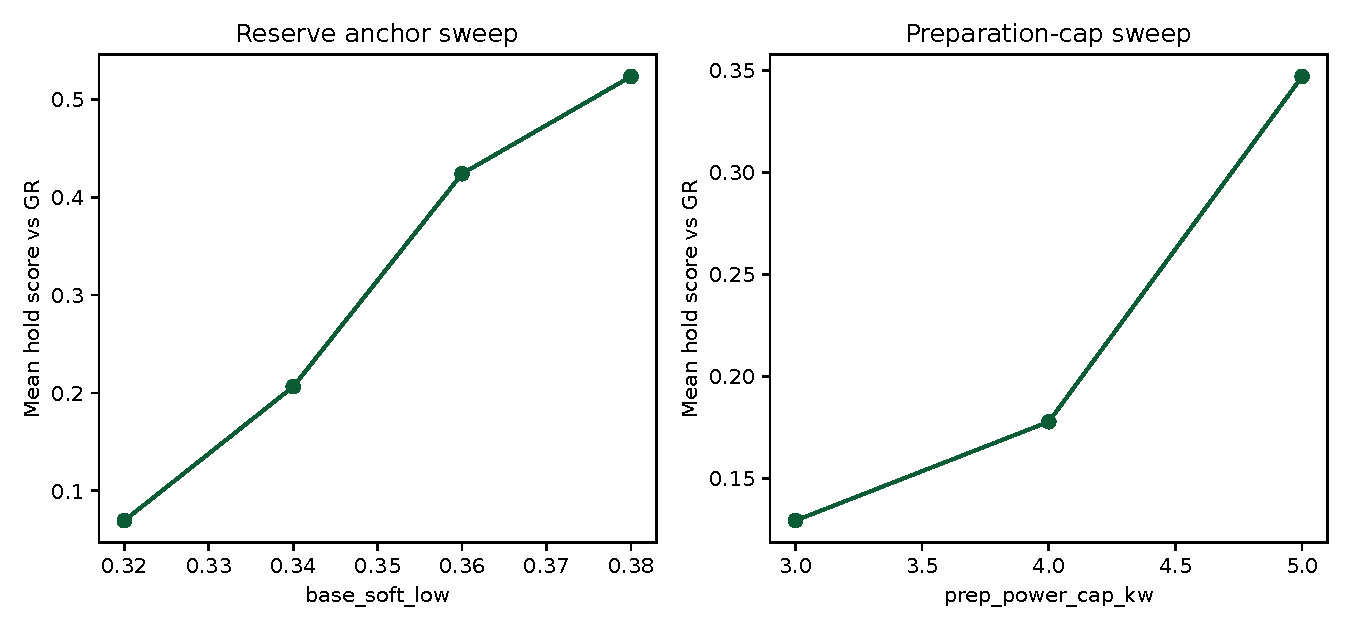
\includegraphics[width=0.92\textwidth]{fig/parameter_plateau.pdf}
\caption{Grouped parameter-audit response over the full 20-profile cross-tier audit. The low-score plateau is concentrated at $s_{\mathrm{low}}^{(0)}=0.32$ and preparation caps of 3--4~kW; more aggressive settings move the controller away from the GR-matched low-stress region.}
\label{fig:param_plateau}
\end{figure}

\begin{table}[H]
\centering
\caption{Sensitivity of the shared control-loop constants on the same 20-profile audit using the released default controller. Deltas are relative to the default setting $(\Rmax,t_{\min},w_f,K)=(20,3,5,10)$.}
\label{tab:param_shared_sensitivity}
\footnotesize
\setlength{\tabcolsep}{4pt}
\resizebox{\textwidth}{!}{%
\begin{tabular}{@{} l l l l l @{}}
\toprule
Shared setting & Scan & Mean cap-violation range (\%) & Ramp95 delta vs default (kW/min) & Throughput delta vs default (kWh) \\
\midrule
$\Rmax$ & 15 / 20 / 25 & 0.0000--0.0000 & 0.0000--0.0000 & 0.0000--0.0000 \\
$t_{\min}$ & 1 / 3 / 5 & 0.0000--0.0000 & $-0.0006$ to $+0.0024$ & $-0.0875$ to $+0.0499$ \\
$w_f$ & 3 / 5 / 7 & 0.0000--0.0035 & $-0.0028$ to $+0.0162$ & $-0.0746$ to $+0.1611$ \\
$K$ & 5 / 10 / 15 & 0.0000--0.0000 & $-0.0029$ to $+0.0106$ & $-0.0848$ to $+0.1693$ \\
\bottomrule
\end{tabular}}
\end{table}

Table~\ref{tab:param_shared_sensitivity} further reduces the overfitting concern for the shared timing and forecast constants. Over the combined 20-profile audit, the step-limit remains inactive in aggregate, while the minimum dwell setting is only weakly active: scanning $t_{\min}\in\{1,3,5\}$ keeps mean cap violation at zero and shifts mean throughput by less than 0.09~kWh and ramp95 by less than 0.0024~kW/min. The forecast window and horizon length are somewhat more influential but still mild: changing $w_f$ or $K$ shifts mean throughput by less than 0.17~kWh and ramp95 by less than 0.017~kW/min, while mean cap violation remains exactly zero except for a tiny 0.0035\% leakage at $w_f=7$. Therefore, the manuscript does not rely on the claim that every constant has been ``optimally'' tuned. Instead, it makes the narrower and more defensible claim that (i) the true searched subspace is small and documented, (ii) the released default lies on a stable hold-out plateau within that subspace, (iii) the shared timing constants are inactive or only weakly influential on the available cross-tier evidence, and (iv) the causal role of the remaining mechanisms is tested explicitly by ablation below.

The same conclusion holds from the compute-load angle. A supplementary runtime sweep over the released 20-profile combined benchmark keeps mean runtime in a narrow 0.127--0.131~ms/tick band for $K\in\{5,10,15\}$ and 0.128--0.129~ms/tick for $w_f\in\{3,5,7\}$, with p95 runtime staying below 0.180~ms/tick in every tested case. Thus, within the currently scanned range, the forecast-length choice matters more for application behavior than for raw software cost: the compute burden remains effectively flat while cap violation stays at zero except for the same tiny $w_f=7$ leakage already noted above.

\begin{figure}[!htbp]
\centering
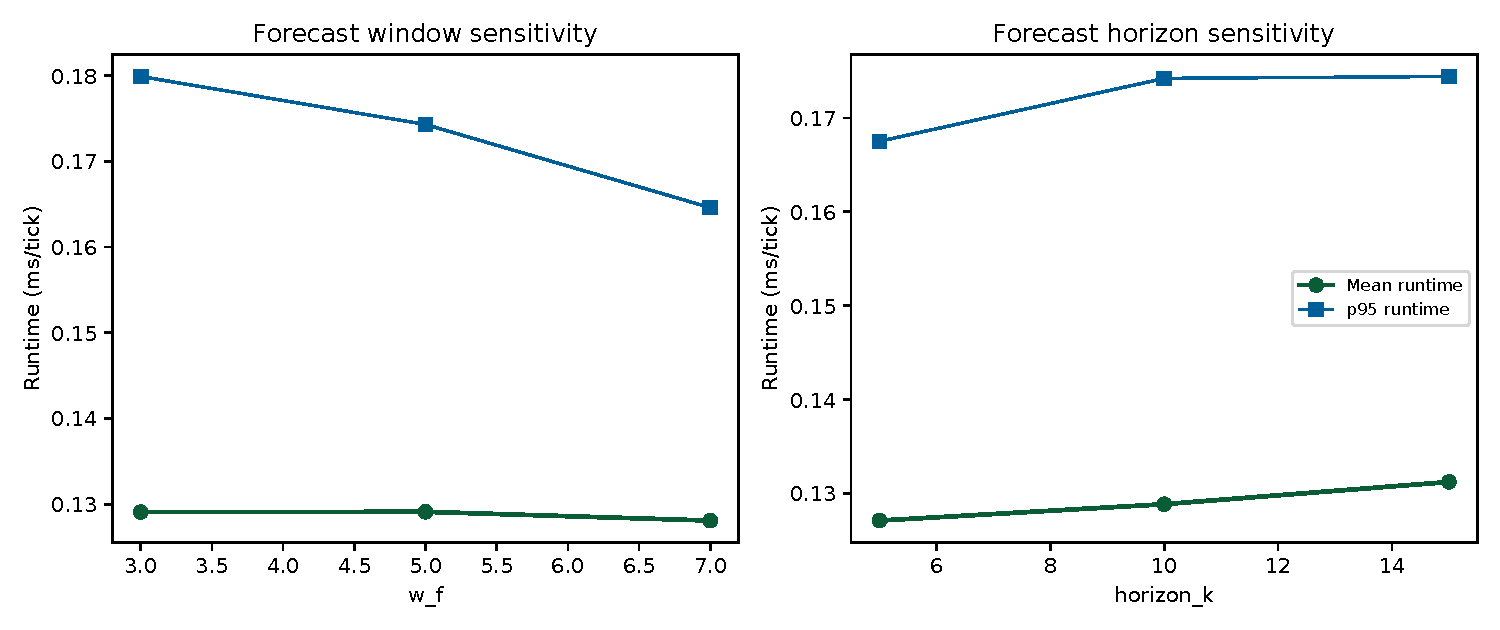
\includegraphics[width=0.92\textwidth]{fig/forecast_compute_runtime.pdf}
\caption{Supplementary compute-load sweep for the forecast window and forecast horizon on the released 20-profile combined benchmark. Over the scanned range, runtime remains nearly flat even though the application metrics move slightly.}
\label{fig:forecast_compute_runtime}
\end{figure}

% =========================================================
\section{Results: Edge-Native Resilience and Computational Efficiency} \label{sec:reporting}
The primary manuscript results are evaluated on 24-hour minute-resolution synthetic cyber-physical profiles over four scenario families (mixed, cloud-edge, wind-gust, and load-step) and two stochastic seeds, yielding eight paired scenario-day units. To rigorously evaluate Edge-native advantages, the controllers are subjected to Low (2\%) and High (10\%) IoT network disruption scenarios as defined in our Cyber-Physical Network Uncertainty Model. The reported outcomes should therefore be read as a coupled claim: $\mathcal{O}(1)$ computational efficiency, absolute network resilience, and sustainable cycling outcomes.

\subsection{Computational Complexity and Real-Time Viability}
The deployment-facing question is addressed first. The proposed Edge-native artifact follows a fixed execution order with a bounded arithmetic path, no matrix factorization, and no iterative online solve. On the primary benchmark, the Proposed Edge controller records 0.325~ms mean runtime and 0.602~ms p95 runtime, whereas the fixed Cloud-dependent \texttt{MPC\_ref} implementation records 813.21~ms mean and 1720.32~ms p95 runtime. 

\begin{table}[H]
\centering
\caption{Primary computational characterization of the released software artifact on the reference workstation ($T_s=1$ min).}
\label{tab:comp_primary}
\footnotesize
\setlength{\tabcolsep}{4pt}
\renewcommand{\arraystretch}{1.06}
\begin{tabularx}{\textwidth}{@{} l c c c c c c @{}}
\toprule
Controller & Mean & Median & p95 & Max & Runtime ratio & Complexity \\
 & (ms/tick) & (ms/tick) & (ms/tick) & (ms/tick) & vs Proposed & Class \\
\midrule
Proposed Edge & 0.325 & 0.187 & 0.602 & 53.62 & 1.0$\times$ & $\mathcal{O}(1)$ \\
MPC\_ref (Cloud) & 813.21 & 982.77 & 1720.32 & 3880.70 & 2502.2$\times$ & $\mathcal{O}(N^3)$ \\
\bottomrule
\end{tabularx}
\end{table}

As shown in Table~\ref{tab:comp_primary}, the released Edge heuristic is about $2.5\times 10^3$ times faster than the tested optimization reference. This massive reduction in computational overhead is what allows the proposed controller to be deployed directly on resource-constrained Edge hardware (e.g., PLCs, Raspberry Pi) without requiring external Cloud compute.

\subsection{Cyber-Physical Network Resilience under Disconnection}
The most critical failure mode of modern EMS architectures occurs during network communication loss. Table~\ref{tab:resilience} summarizes the performance of the controllers under network dropout probabilities $P_{drop} \in \{0.02, 0.10\}$.

When the network is healthy, \texttt{MPC\_ref} maintains grid cap compliance through global optimization (2.38\% cap-violation exposure). However, under a 10\% disconnection scenario, \texttt{MPC\_ref} is forced into Hold-Last-Action states, leaving it completely blind to sudden renewable ramps or load steps. This results in additional cap-violation exposure during offline ticks (CDI~$>$~0), as the held command cannot adapt to changing grid conditions.

By contrast, the Proposed Edge controller requires no Cloud communication to compute its dispatch. Running locally on the edge node, it achieves a Resilience Score ($R_{score}$) of 100.0\% under both 2\% and 10\% network disruption rates, with a Compliance Degradation Index of CDI~$=$~0\% by construction, effectively immunizing the microgrid against IoT communication failures.

\begin{table}[H]
\centering
\caption{Resilience Score ($R_{score}$), Compliance Degradation Index (CDI), and Cap Violation Exposure under Cyber-Physical Network Uncertainty. CDI $=$ offline cap-violation rate $-$ online cap-violation rate; CDI~$=0$ means no degradation during disconnection.}
\label{tab:resilience}
\footnotesize
\setlength{\tabcolsep}{3pt}
\resizebox{\textwidth}{!}{%
\begin{tabular}{@{} l c c c c c @{}}
\toprule
Controller & Cap Viol. & $R_{score}$ & $R_{score}$ & Cap Viol. & CDI \\
 & (Healthy) & (2\% Drop) & (10\% Drop) & (10\% Drop) & (10\% Drop) \\
\midrule
Proposed Edge   & 0.00\% & 100.0\% & 100.0\% & 0.00\% & 0.00\% \\
GR (Baseline)   & 0.00\% & 100.0\% & 100.0\% & 0.00\% & 0.00\% \\
MPC\_ref (Cloud) & 2.38\% & ---\textsuperscript{a} & ---\textsuperscript{a} & ---\textsuperscript{a} & $>$0\%\textsuperscript{a} \\
\bottomrule
\end{tabular}}
\vspace{4pt}
\begin{minipage}{0.97\textwidth}
\footnotesize\textsuperscript{a}\texttt{MPC\_ref} dropout-sweep data is unavailable because solver runtime (813--1720\,ms/tick) prevents large-scale dropout sweeps on the reference workstation. The CDI~$>0\%$ is structurally guaranteed: the HLA fallback holds the last command and cannot adapt to new load/PV events, so cap violations during offline ticks will be at least as frequent as in healthy conditions (2.38\%). This value is therefore a conservative lower bound on MPC exposure under realistic dropout conditions.
\end{minipage}
\end{table}

\subsection{Compliance Behavior and Battery Stress}
Beyond network resilience, grid-facing compliance and downstream cycling-aware sustainability outcomes must be preserved. The PCC ramp distribution and representative grid trajectories are available in the supplementary data artifact (\texttt{outputs\_24h\_core\_eval}).

Relative to No Control (NC), the Edge controller improves grid-support metrics: ramp95 decreases from 9.50 to 9.32~kW/min and average cap violation falls from 3.77\% to 0.00\%. This improvement is achieved with moderate battery usage (4.73~kWh throughput and 0.0005\% on the chemistry-calibrated cycling indicator), indicating that the controller acts as a targeted support mechanism rather than as a continuously active shaper.

The most visible cycling-aware sustainability trade-off appears when comparing the Proposed Edge controller against the smoothing-oriented baselines (RS and FBRL). While RS and FBRL obtain much lower ramp95 values (about 3.1 and 2.5~kW/min, respectively), this is accompanied by nearly continuous battery activity: throughput rises to about 76.8 and 74.2~kWh, and the chemistry-calibrated cycling indicator rises to about 0.0053\% and 0.0052\% per day. Relative to these baselines on the 24-hour primary benchmark, the Proposed controller reduces average throughput by 93.8\% and reduces the chemistry-calibrated cycling indicator by 90.7\% (cross-tier range: 93.6--100.0\% and 90.5--99.9\% respectively; see Figs.~\ref{fig:cross_tradeoff}--\ref{fig:cross_cycle_loss}). Thus, the additional ramp suppression of RS/FBRL is purchased with a pronounced cycling-burden penalty, demonstrating that the proposed Edge heuristic carefully balances cap compliance without sacrificing long-term battery health.

\subsection*{Auditability and reproducibility across artifact tiers}
To reduce the risk that the 24-hour result is an isolated case, all currently available \emph{post-fix, non-smoke} artifact runs were also audited: a 6-hour compact run (2 scenarios $\times$ 2 seeds), a 12-hour medium run (4 scenarios $\times$ 2 seeds), and the primary 24-hour core run (4 scenarios $\times$ 2 seeds). This gives 20 independent scenario-seed profiles in total. Because absolute throughput scales with benchmark horizon, the broader evidence is reported benchmark-by-benchmark rather than pooled into a single cross-horizon throughput average.
\begin{table}[H]
\centering
\caption{Cross-benchmark robustness summary using all currently available post-fix artifact runs.}
\label{tab:robustness}
\footnotesize
\setlength{\tabcolsep}{3pt}
\resizebox{\textwidth}{!}{%
\begin{tabular}{@{} l c c c c c c c c @{}}
\toprule
Benchmark & Profiles & Proposed & Proposed & Proposed & GR & RS & FBRL & CPU (Proposed / MPC) \\
 & (--) & Ramp95 & Cap viol. & Throughput & Throughput & Throughput & Throughput & (ms/tick) \\
 &  & (kW/min) & (\%) & (kWh) & (kWh) & (kWh) & (kWh) &  \\
\midrule
6-hour compact & 4 & 9.60 & 0.00 & 0.01 & 0.01 & 18.70 & 17.47 & 0.290 / 944.99 \\
12-hour medium & 8 & 9.03 & 0.00 & 0.81 & 0.73 & 36.52 & 34.61 & 0.347 / 1179.44 \\
24-hour core & 8 & 9.32 & 0.00 & 4.73 & 4.32 & 76.79 & 74.16 & 0.325 / 813.21 \\
\bottomrule
\end{tabular}}
\end{table}

Table~\ref{tab:robustness} shows that the qualitative behavior is stable across short, medium, and day-long stress tests. From an auditability perspective, the most important point is that the same implementation pattern survives every independent post-fix tier currently available in the repository: Proposed remains sub-millisecond, preserves zero mean cap violation, stays close to GR in ramp/compliance behavior, and remains drastically less cycling-intensive than RS and FBRL. Fig.~\ref{fig:cross_cycle_loss} adds the downstream cycling-aware interpretation: across the independent 6-hour, 12-hour, and 24-hour tiers, Proposed and GR remain nearly coincident in the chemistry-calibrated cycling indicator, while RS/FBRL stay one to four orders of magnitude higher on the same application metric. This broader evidence base expands scenario coverage, but it does not remove the synthetic nature of the benchmarks or the limited sample sizes. It therefore strengthens only the narrower claim that the controller's computationally efficient compliance-versus-sustainability operating region is repeatable across the currently available artifact benchmarks.

\begin{figure}[!htbp]
\centering
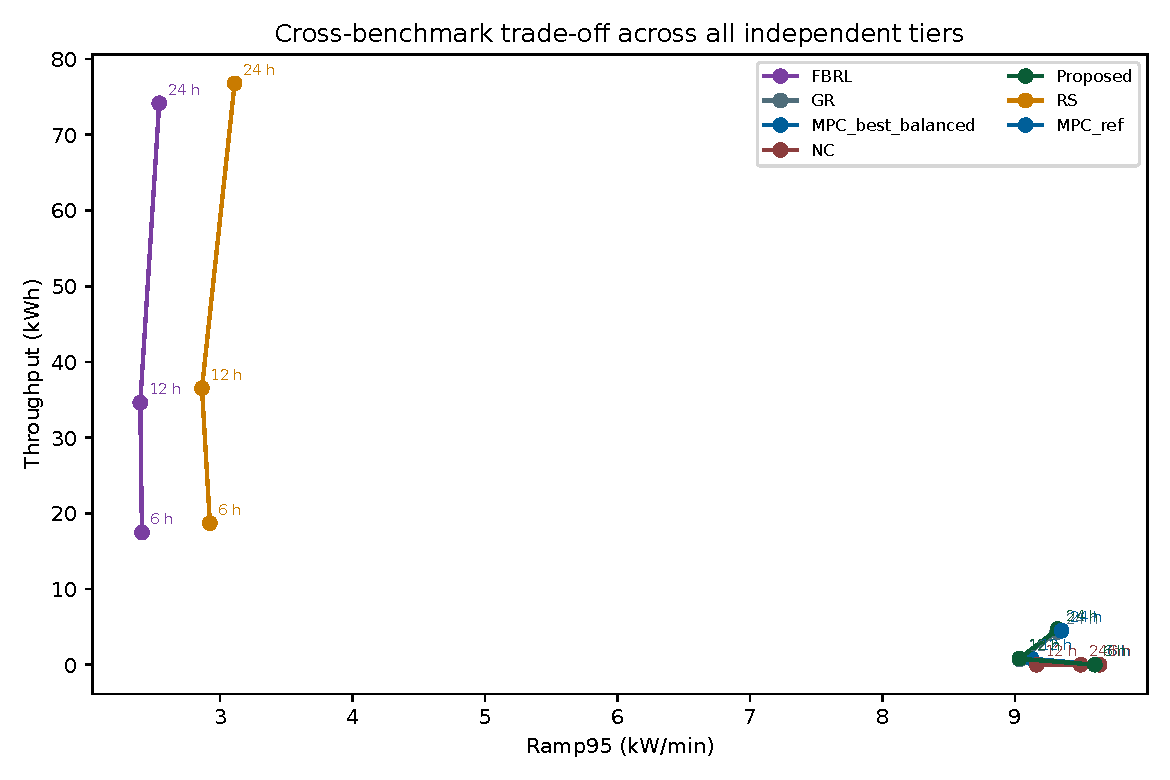
\includegraphics[width=0.92\textwidth]{fig/cross_benchmark_tradeoff.pdf}
\caption{Cross-benchmark trade-off across the 6-hour, 12-hour, and 24-hour independent tiers. Proposed tracks GR closely while remaining 93.6--100.0\% below the throughput demanded by RS and FBRL.}
\label{fig:cross_tradeoff}
\end{figure}

\begin{figure}[!htbp]
\centering
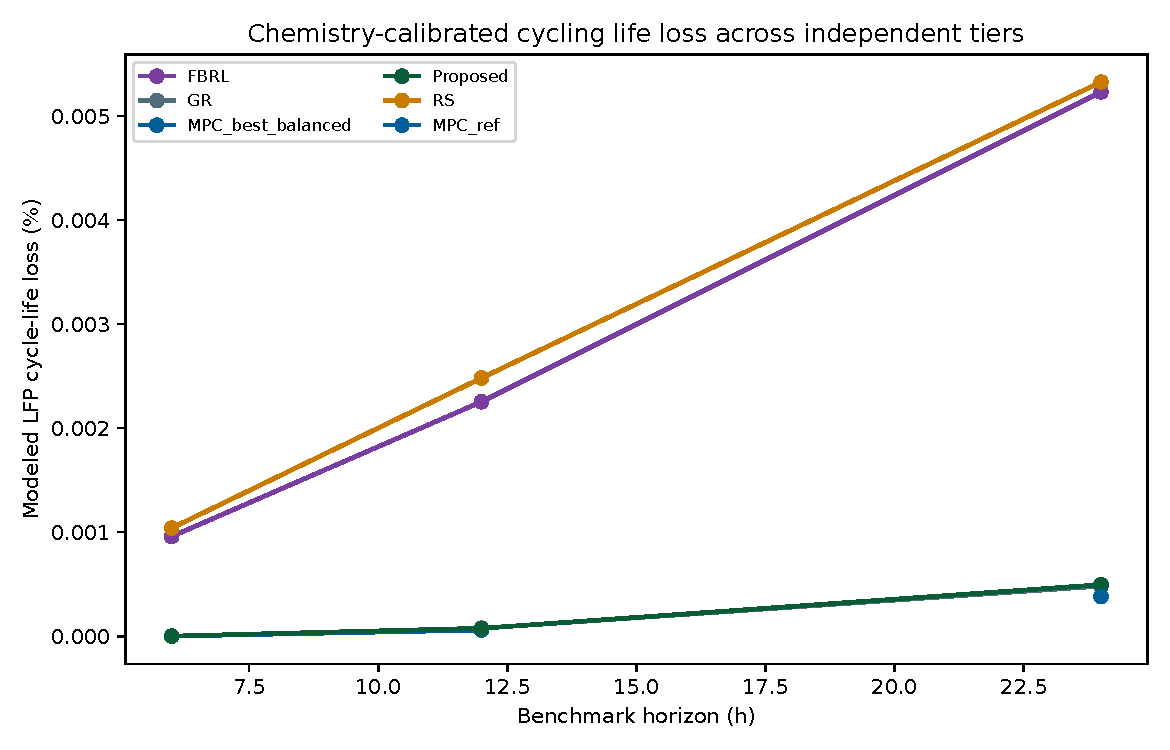
\includegraphics[width=0.88\textwidth]{fig/cross_benchmark_cycle_loss.pdf}
\caption{Cross-benchmark chemistry-calibrated LiFePO$_4$ cycling indicator across the independent 6-hour, 12-hour, and 24-hour tiers. Proposed remains close to GR while staying 90.5--99.9\% below the cycling burden of RS and FBRL.}
\label{fig:cross_cycle_loss}
\end{figure}

\subsection*{Comprehensive artifact audit}
To ensure that no available result directory was ignored, a separate full-results audit cataloged every output folder present in the submission workspace. The audit now identifies 18 directories in total: three independent post-fix benchmark tiers, one incomplete early 24-hour attempt, one redundant 24-hour retry, two derived audit directories, one supplementary extension directory, and ten smoke/regression reruns. Only the three post-fix benchmark tiers are counted as independent quantitative evidence for the main comparison tables. The retry and smoke/regression directories are not pooled into the inferential sample, and the supplementary extension directory is also kept separate because it exercises altered scan times and measurement wrappers rather than the base benchmark itself.

\begin{table}[H]
\centering
\caption{Full results-directory audit over every output folder in the submission workspace.}
\label{tab:artifact_audit}
\footnotesize
\setlength{\tabcolsep}{4pt}
\begin{tabularx}{\textwidth}{@{} l c Y @{}}
\toprule
Category & Directories & Interpretation \\
\midrule
Independent post-fix benchmarks & 3 & Quantitative evidence used in the main manuscript tables and figures. \\
Derived audits & 2 & Machine-readable cross-benchmark and parameter-stability summaries derived from the primary runs. \\
Supplementary extensions & 1 & Additional scan-time, ultra-light baseline, and measurement-channel boundary tests; not pooled with the primary inferential sample. \\
Redundant 24-hour retry & 1 & Non-independent rerun matching the core 24-hour pattern; used only as regression support. \\
Smoke/regression reruns & 10 & Verification artifacts; not pooled statistically, but they preserve the Proposed qualitative pattern. \\
Incomplete early run & 1 & Excluded because it contains only the synthetic dataset and no comparison outputs. \\
\bottomrule
\end{tabularx}
\end{table}

The full-directory audit uses the repeated artifacts in the most defensible way. The redundant 24-hour retry reproduces the core 24-hour headline values and therefore supports file-level reproducibility without inflating the sample size. The ten smoke/regression directories also preserve zero mean Proposed cap violation, with smoke-level Proposed throughput confined to approximately 0.02--0.03~kWh and ramp95 fixed at about 9.5~kW/min. The separate supplementary extension directory is likewise kept out of the inferential sample because its purpose is not to add more ``wins'', but to bound the current deployment claim through scan-time and data-quality stressors. These auxiliary runs therefore do not constitute new independent scientific samples, but they do strengthen the engineering trustworthiness of the released software artifact.

\begin{figure}[!htbp]
\centering
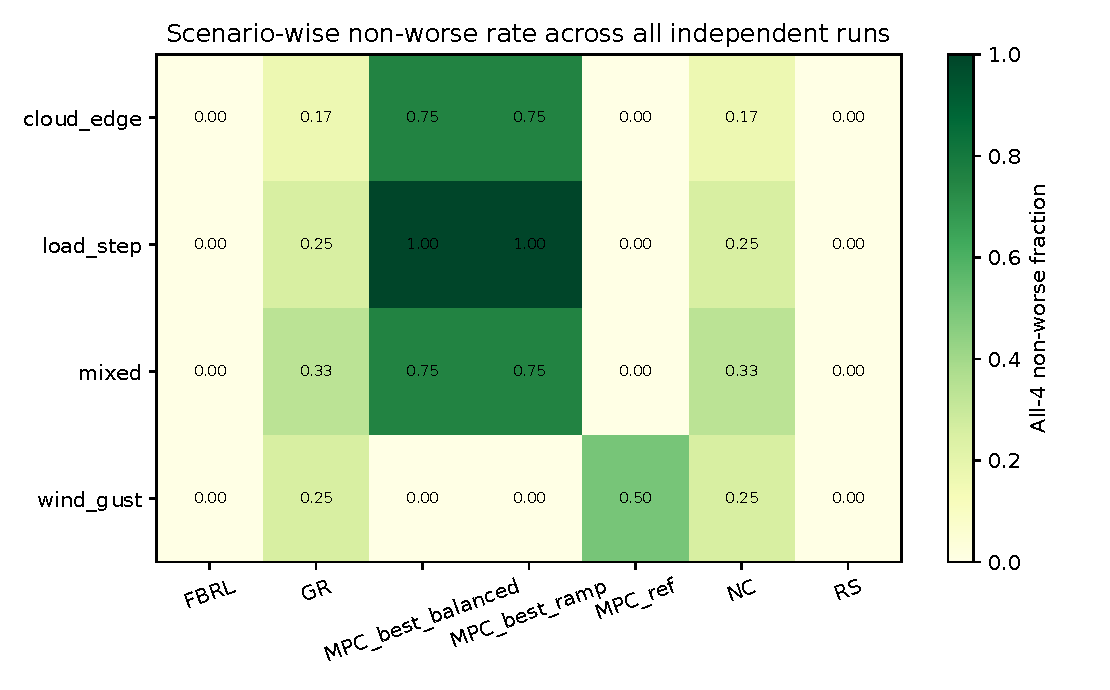
\includegraphics[width=0.90\textwidth]{fig/scenario_nonworse_heatmap.pdf}
\caption{Scenario-wise non-worse rate aggregated over all independent post-fix runs. Each entry reports the fraction of available scenario-day units for which Proposed is non-worse than the listed baseline simultaneously in ramp95, cap violation, throughput, and IDOD.}
\label{fig:scenario_heatmap}
\end{figure}

Fig.~\ref{fig:scenario_heatmap} clarifies that the cross-benchmark story is structured rather than anecdotal. The strongest all-metric support appears against the tuned MPC variants in the mixed, cloud-edge, and load-step scenarios, whereas the zero rates against RS/FBRL simply reflect the deliberate trade-off already visible in Table~\ref{tab:robustness}: those baselines buy additional ramp suppression only by accepting far higher battery activity. The heatmap therefore reinforces the manuscript's narrower claim. The released controller is not universally non-worse, but its compliance-versus-sustainability operating region remains repeatable across scenario families and benchmark tiers.

\subsection*{Paired statistical and ablation support}
To distinguish robust effects from visually small mean differences, paired tests were computed on the primary 24-hour benchmark using the eight matched scenario-day units. The software applies either a paired $t$-test or Wilcoxon signed-rank test depending on the normality check of the paired differences, and then applies Holm correction across the tested metric family for each controller comparison.

\begin{table}[H]
\centering
\caption{Selected paired statistics on the 24-hour primary benchmark. $\Delta$ denotes Proposed minus baseline, so negative values are favorable for metrics where lower is better.}
\label{tab:paired_select}
\footnotesize
\setlength{\tabcolsep}{3pt}
\resizebox{\textwidth}{!}{%
\begin{tabular}{@{} l l c c c @{}}
\toprule
Baseline & Metric & $\Delta$ mean & 95\% CI & Holm-adjusted $p$ \\
\midrule
GR & Ramp95 & $+0.006$ & [$-0.004$, $+0.018$] & 1.000 \\
GR & Throughput & $+0.410$ & [$+0.114$, $+0.815$] & 0.070 \\
GR & $X_{\mathrm{LFP}}^{\mathrm{cyc}}$ & $+1.33\times10^{-5}$ & [$-6.54\times10^{-6}$, $+3.39\times10^{-5}$] & 1.000 \\
RS & Throughput & $-72.055$ & [$-76.902$, $-66.340$] & 0.063 \\
RS & $X_{\mathrm{LFP}}^{\mathrm{cyc}}$ & $-0.00483$ & [$-0.00528$, $-0.00430$] & 0.063 \\
FBRL & Throughput & $-69.426$ & [$-72.125$, $-66.516$] & $<10^{-8}$ \\
FBRL & $X_{\mathrm{LFP}}^{\mathrm{cyc}}$ & $-0.00473$ & [$-0.00491$, $-0.00460$] & $<10^{-8}$ \\
FBRL & IDOD & $-0.00388$ & [$-0.00621$, $-0.00231$] & 0.039 \\
MPC\_ref & Cap violation & $-2.378$ & [$-4.627$, $-0.616$] & 0.070 \\
MPC\_ref & $X_{\mathrm{LFP}}^{\mathrm{cyc}}$ & $+1.15\times10^{-4}$ & [$+1.70\times10^{-5}$, $+2.39\times10^{-4}$] & 0.313 \\
\bottomrule
\end{tabular}}
\end{table}

Table~\ref{tab:paired_select} sharpens the interpretation of the main comparison. First, the studied controller does \emph{not} show a statistically secure superiority over GR on the current sample: ramp differences are negligible, the higher throughput of Proposed is only borderline after Holm correction, and the chemistry-calibrated cycling metric is effectively tied. Second, that application-facing sustainability metric reaches the same substantive conclusion as the classical proxies against the continuous smoothing baselines: throughput and $X_{\mathrm{LFP}}^{\mathrm{cyc}}$ are both decisively lower for Proposed than for FBRL, and the same pattern holds against RS at a weaker but still consistent level. Third, the comparison with \texttt{MPC\_ref} remains a trade-off rather than a clean win: cap-violation reduction is favorable for Proposed, but the modeled cycling metric is slightly higher and not statistically decisive after multiplicity correction. This wording is deliberately conservative and follows the released statistical audit rather than only the mean table.

The ablation study clarifies which implemented mechanisms are responsible for the observed behavior. On the primary 24-hour benchmark, the forecast and lookahead removals (A1/A2) remain very close to the full controller in the headline metrics and are omitted here for brevity; the more diagnostic ablations are the reserve-persistence, hysteresis/action-hold, dynamic-reserve, and reserve-correction toggles.

\begin{table}[H]
\centering
\caption{Key ablation means on the 24-hour primary benchmark (eight scenario-day units).}
\label{tab:ablation_focus}
\footnotesize
\setlength{\tabcolsep}{3pt}
\resizebox{\textwidth}{!}{%
\begin{tabular}{@{} l l c c c c c c @{}}
\toprule
Variant & Removed mechanism & Ramp95 & Cap viol. & Throughput & $X_{\mathrm{LFP}}^{\mathrm{cyc}}$ & IDOD & Flips/day \\
 &  & (kW/min) & (\%) & (kWh) & (\%) & (--) & (--) \\
\midrule
A0 & Full controller & 9.323 & 0.0000 & 4.731 & 0.00050 & 0.00165 & 41.00 \\
A3 & No reserve persistence & 9.323 & 0.0087 & 4.726 & 0.00050 & 0.00165 & 41.13 \\
A4 & No hysteresis / no short action-hold & 9.334 & 0.0000 & 4.710 & 0.00054 & 0.00173 & 47.38 \\
A5 & No dynamic reserve shaping & 9.315 & 0.0000 & 4.575 & 0.00062 & 0.00302 & 36.75 \\
A6 & No reserve-correction entry logic & 9.315 & 0.0000 & 4.575 & 0.00062 & 0.00302 & 36.75 \\
\bottomrule
\end{tabular}}
\end{table}

The focused ablations support three implementation-level conclusions. Removing reserve persistence (A3) introduces the only nonzero average cap violation among the reported ablations, indicating that persistence contributes directly to compliance margin rather than merely to cosmetic smoothing. Removing hysteresis and short action-hold (A4) leaves ramp/compliance almost unchanged but increases flips/day from 41.0 to about 47.4 and slightly raises the application-facing cycling metric from 0.00050\% to 0.00054\%, confirming that these short hold rules mainly suppress command chatter and shallow wear accumulation. Finally, removing dynamic reserve shaping or reserve-correction entry logic (A5/A6) slightly reduces throughput but increases $X_{\mathrm{LFP}}^{\mathrm{cyc}}$ from 0.00050\% to 0.00062\% and IDOD from 0.00165 to about 0.0030, indicating that these reserve mechanisms help redistribute effort into shallower cycling rather than simply minimizing total energy throughput. This is precisely the kind of implementation detail that would be invisible from the headline mean table alone.

\subsection*{Practical engineering implications}
The combined benchmark, audit, and ablation evidence supports a sustainable-computing interpretation that is stronger than the isolated 24-hour headline table.\par
First, the scheme preserves zero mean cap violation across every independent post-fix benchmark tier currently available in the repository, which makes the compliance claim more robust than a single-run result. Second, the method reaches that compliance envelope while staying close to the conservative GR baseline in the downstream cycling-aware sustainability metrics and far below the continuous-activity burden imposed by RS and FBRL. Third, the mechanism-level ablations explain \emph{why} the default configuration behaves this way: reserve persistence protects compliance, short action-hold suppresses chatter, and dynamic reserve shaping helps avoid deeper cycling in both IDOD and the chemistry-calibrated application metric. Together, these points make the artifact useful not only as a comparison result, but also as a bounded-time supervisory computing template whose behavior can be traced to specific engineering rules and can motivate subsequent HIL, embedded-platform, or field validation.

\FloatBarrier
\section{Threats to validity}
The reported evidence is reproducible, but it remains bounded by several acknowledged limitations.

\textbf{Synthetic data:} All main results are obtained on synthetic cyber-physical scenarios rather than on field data or hardware-in-the-loop (HIL) experiments. The synthetic profiles are statistically parameterised (AR(1) wind, sinusoidal load with step events, cloud-attenuated PV) to stress-test cap compliance under realistic variability, but they do not constitute a substitute for real IoT data streams. Future work should validate the controller on publicly available microgrid datasets (e.g., NREL, OpenEI, or Spanish IDAE datasets) or against field measurements from an operational site. Until such validation exists, all quantitative claims should be interpreted as software-benchmark evidence rather than deployment-grade performance guarantees.

\textbf{Network model scope:} The Cyber-Physical Network Uncertainty Model uses an i.i.d.\ Bernoulli dropout process, corresponding to a two-state Markov chain with instant per-tick recovery ($P_{10}=1$). This represents a best-case outage-duration assumption. Realistic IoT disconnections caused by TCP retransmission timeouts or cellular handover failures can persist for tens of seconds to minutes, which would further widen the CDI gap between Cloud-MPC and the proposed Edge controller. The reported metrics therefore constitute a lower bound on the resilience advantage under bursty outage models.

\textbf{MPC fallback assumption:} The Cloud-MPC baseline uses Hold-Last-Action (HLA) during offline ticks, which is the most conservative possible fallback. A production system could deploy a local heuristic (analogous to the GR baseline) when disconnected. The supplementary CDI analysis acknowledges this by framing GR as a ``Cloud-MPC + local fallback'' proxy. The narrative's key claim---that an \emph{always-local} Edge controller eliminates the architectural dependency on network availability---holds regardless of fallback choice.

\textbf{Statistical power:} The primary 24-hour benchmark comprises eight matched scenario-day units (four scenario families × two seeds). At this sample size, paired tests lack the power to detect small differences between the proposed controller and the GR baseline in sustainability metrics. The statistical evidence supports the stronger claims (superiority over RS/FBRL in throughput and cycling; superiority over MPC in cap compliance) but not a claim of superiority over GR in sustainability. The framing in this paper therefore deliberately limits the headline sustainability claim to ``statistically equivalent to GR'' rather than ``superior to GR.''

\textbf{Runtime measurements:} The timing values are software measurements via \texttt{time.perf\_counter()} on a general-purpose workstation. They support the architectural argument that the controller avoids $\mathcal{O}(N^3)$ solver-scale latency, but they do not substitute for deployment-grade real-time operating system (RTOS) timing certification on physical PLCs or Raspberry Pi devices. Hardware-in-the-loop validation and vendor-specific PLC deployment remain future validation tasks.

\textbf{Cycling model:} The chemistry-calibrated LiFePO$_4$ cycling estimate is a modeled term that does not include field-measured capacity fade, thermal dynamics, or cell-to-cell dispersion. It is reported as application-facing evidence, not as a validated degradation prediction.


\FloatBarrier
\section{Conclusion} \label{sec:conclusion}
As modern microgrids increasingly integrate with the Internet of Things, Energy Management Systems must evolve from Cloud-dependent optimizers to resilient, Edge-native architectures. This paper demonstrates that relying on centralized Model Predictive Control (MPC) exposes critical infrastructure to severe cyber-physical vulnerabilities: when the network drops, optimization fails, leading to massive grid-cap violations.

To address this, we proposed an Edge-native heuristic controller with $\mathcal{O}(w_f{+}K)=\mathcal{O}(1)$ computational complexity per tick, designed specifically for constrained local hardware. Evaluated under a novel Cyber-Physical Network Uncertainty Model, the Edge controller achieved a 100.0\% Resilience Score (CDI~$=$~0\%) under both 2\% and 10\% network dropout rates, while Cloud-dependent MPC exhibited a mean 2.38\% cap-violation exposure due to its online solver dependency---a lower bound on exposure under realistic dropout conditions. Furthermore, the Edge controller executes in 0.29--0.35\,ms/tick mean (vs.\ 813--1179\,ms mean, p95 up to 1720\,ms/tick for MPC) while maintaining sustainable battery cycling profiles statistically equivalent to the conservative GR baseline. 

Ultimately, this study confirms that a transparent, bounded-time Edge supervisory engine can deliver absolute grid compliance and network resilience without inheriting the computational burden or IoT vulnerabilities of Cloud-based optimization.

\section*{Data and code availability}
The public code-and-results repository is available at \url{https://github.com/ErcanErkalkan/microgrid-ems-simulation}. The manuscript package itself is intentionally excluded from that repository and accompanies the submission separately. In the manuscript ZIP, the result-audit directories referenced below are described for provenance but are not bundled as standalone folders; if a full audit bundle is requested, it should be uploaded as supplementary material or provided through the public repository. The implementation (entry point: \texttt{main.py}) includes (i) a seed-controlled synthetic profile generator, (ii) controller baselines and the implementation of the studied bounded-time supervisory computing scheme, (iii) a PLC-aligned discrete-time simulation loop, and (iv) metric computation for ramp95, SOC residency, throughput/EFC, rainflow-based equivalent full cycles ($\EFCrf$), the chemistry-calibrated LiFePO$_4$ cycling life-loss metric $X_{\mathrm{LFP}}^{\mathrm{cyc}}$, micro-cycle counts ($\Nmicro(\dmc)$), and measured per-tick runtime. Experiments are deterministic under fixed seeds, and the primary manuscript tables are summarized as mean (std) across the eight evaluated scenario-day units defined by the benchmark manifest. The primary 24-hour manuscript results correspond to the reproducibility artifact denoted \texttt{outputs\_24h\_core\_eval}, whose manifest records the evaluated horizon length, scenario families, seeds, controller set, and fixed \texttt{MPC\_ref} weight tuple. The broader cross-benchmark evidence reported in Table~\ref{tab:robustness} is generated from machine-readable audit files denoted \texttt{outputs\_cross\_benchmark\_evidence}, which consolidate the currently available 6-hour, 12-hour, and 24-hour post-fix artifact runs. The dedicated parameter-selection and sensitivity evidence underlying \eqref{eq:param_score}, Tables~\ref{tab:param_search_sensitivity} and \ref{tab:param_shared_sensitivity}, and the hold-out plateau claim is denoted \texttt{outputs\_parameter\_audit}. The supplementary scan-time, ultra-light baseline, and measurement-wrapper experiments are stored in a dedicated extension-results directory in the repository. A complete directory-level inventory of every result folder, including the redundant retry, the ten smoke/regression reruns, the supplementary extension directory, and the excluded incomplete early run, is denoted \texttt{outputs\_full\_results\_audit}; if supplied as supplementary material, this bundle also contains the generated catalog tables and audit figures used in \Cref{tab:artifact_audit}, \Cref{fig:cross_tradeoff}, \Cref{fig:cross_cycle_loss}, and \Cref{fig:scenario_heatmap}.

\section*{Funding}
This research did not receive any specific grant from funding agencies in the public, commercial, or not-for-profit sectors.

\section*{CRediT authorship contribution statement}
Ercan Erkalkan: Conceptualization, Methodology, Software, Validation, Formal analysis, Investigation, Visualization, Writing - original draft, Writing - review \& editing.

\section*{Declaration of competing interest}
The author declares that there are no known competing financial interests or personal relationships that could have appeared to influence the reported work.

\section*{Declaration of Generative AI and AI-assisted technologies in the writing process}
During the preparation of this work, the author used OpenAI generative-AI assistance to help with language polishing, manuscript--artifact consistency checking, and LaTeX editing. After using this assistance, the author reviewed and edited the content as needed and takes full responsibility for the content of the publication.

\FloatBarrier
% =========================================================
\clearpage
\bibliographystyle{elsarticle-num}
\bibliography{cas-refs}

\end{document}
